% Options for packages loaded elsewhere
% Options for packages loaded elsewhere
\PassOptionsToPackage{unicode}{hyperref}
\PassOptionsToPackage{hyphens}{url}
\PassOptionsToPackage{dvipsnames,svgnames,x11names}{xcolor}
%
\documentclass[
  brazilian,
  letterpaper,
  DIV=11,
  numbers=noendperiod]{scrreprt}
\usepackage{xcolor}
\usepackage[margin=2.5cm]{geometry}
\usepackage{amsmath,amssymb}
\setcounter{secnumdepth}{5}
\usepackage{iftex}
\ifPDFTeX
  \usepackage[T1]{fontenc}
  \usepackage[utf8]{inputenc}
  \usepackage{textcomp} % provide euro and other symbols
\else % if luatex or xetex
  \usepackage{unicode-math} % this also loads fontspec
  \defaultfontfeatures{Scale=MatchLowercase}
  \defaultfontfeatures[\rmfamily]{Ligatures=TeX,Scale=1}
\fi
\usepackage{lmodern}
\ifPDFTeX\else
  % xetex/luatex font selection
\fi
% Use upquote if available, for straight quotes in verbatim environments
\IfFileExists{upquote.sty}{\usepackage{upquote}}{}
\IfFileExists{microtype.sty}{% use microtype if available
  \usepackage[]{microtype}
  \UseMicrotypeSet[protrusion]{basicmath} % disable protrusion for tt fonts
}{}
\makeatletter
\@ifundefined{KOMAClassName}{% if non-KOMA class
  \IfFileExists{parskip.sty}{%
    \usepackage{parskip}
  }{% else
    \setlength{\parindent}{0pt}
    \setlength{\parskip}{6pt plus 2pt minus 1pt}}
}{% if KOMA class
  \KOMAoptions{parskip=half}}
\makeatother
% Make \paragraph and \subparagraph free-standing
\makeatletter
\ifx\paragraph\undefined\else
  \let\oldparagraph\paragraph
  \renewcommand{\paragraph}{
    \@ifstar
      \xxxParagraphStar
      \xxxParagraphNoStar
  }
  \newcommand{\xxxParagraphStar}[1]{\oldparagraph*{#1}\mbox{}}
  \newcommand{\xxxParagraphNoStar}[1]{\oldparagraph{#1}\mbox{}}
\fi
\ifx\subparagraph\undefined\else
  \let\oldsubparagraph\subparagraph
  \renewcommand{\subparagraph}{
    \@ifstar
      \xxxSubParagraphStar
      \xxxSubParagraphNoStar
  }
  \newcommand{\xxxSubParagraphStar}[1]{\oldsubparagraph*{#1}\mbox{}}
  \newcommand{\xxxSubParagraphNoStar}[1]{\oldsubparagraph{#1}\mbox{}}
\fi
\makeatother

\usepackage{color}
\usepackage{fancyvrb}
\newcommand{\VerbBar}{|}
\newcommand{\VERB}{\Verb[commandchars=\\\{\}]}
\DefineVerbatimEnvironment{Highlighting}{Verbatim}{commandchars=\\\{\}}
% Add ',fontsize=\small' for more characters per line
\usepackage{framed}
\definecolor{shadecolor}{RGB}{241,243,245}
\newenvironment{Shaded}{\begin{snugshade}}{\end{snugshade}}
\newcommand{\AlertTok}[1]{\textcolor[rgb]{0.68,0.00,0.00}{#1}}
\newcommand{\AnnotationTok}[1]{\textcolor[rgb]{0.37,0.37,0.37}{#1}}
\newcommand{\AttributeTok}[1]{\textcolor[rgb]{0.40,0.45,0.13}{#1}}
\newcommand{\BaseNTok}[1]{\textcolor[rgb]{0.68,0.00,0.00}{#1}}
\newcommand{\BuiltInTok}[1]{\textcolor[rgb]{0.00,0.23,0.31}{#1}}
\newcommand{\CharTok}[1]{\textcolor[rgb]{0.13,0.47,0.30}{#1}}
\newcommand{\CommentTok}[1]{\textcolor[rgb]{0.37,0.37,0.37}{#1}}
\newcommand{\CommentVarTok}[1]{\textcolor[rgb]{0.37,0.37,0.37}{\textit{#1}}}
\newcommand{\ConstantTok}[1]{\textcolor[rgb]{0.56,0.35,0.01}{#1}}
\newcommand{\ControlFlowTok}[1]{\textcolor[rgb]{0.00,0.23,0.31}{\textbf{#1}}}
\newcommand{\DataTypeTok}[1]{\textcolor[rgb]{0.68,0.00,0.00}{#1}}
\newcommand{\DecValTok}[1]{\textcolor[rgb]{0.68,0.00,0.00}{#1}}
\newcommand{\DocumentationTok}[1]{\textcolor[rgb]{0.37,0.37,0.37}{\textit{#1}}}
\newcommand{\ErrorTok}[1]{\textcolor[rgb]{0.68,0.00,0.00}{#1}}
\newcommand{\ExtensionTok}[1]{\textcolor[rgb]{0.00,0.23,0.31}{#1}}
\newcommand{\FloatTok}[1]{\textcolor[rgb]{0.68,0.00,0.00}{#1}}
\newcommand{\FunctionTok}[1]{\textcolor[rgb]{0.28,0.35,0.67}{#1}}
\newcommand{\ImportTok}[1]{\textcolor[rgb]{0.00,0.46,0.62}{#1}}
\newcommand{\InformationTok}[1]{\textcolor[rgb]{0.37,0.37,0.37}{#1}}
\newcommand{\KeywordTok}[1]{\textcolor[rgb]{0.00,0.23,0.31}{\textbf{#1}}}
\newcommand{\NormalTok}[1]{\textcolor[rgb]{0.00,0.23,0.31}{#1}}
\newcommand{\OperatorTok}[1]{\textcolor[rgb]{0.37,0.37,0.37}{#1}}
\newcommand{\OtherTok}[1]{\textcolor[rgb]{0.00,0.23,0.31}{#1}}
\newcommand{\PreprocessorTok}[1]{\textcolor[rgb]{0.68,0.00,0.00}{#1}}
\newcommand{\RegionMarkerTok}[1]{\textcolor[rgb]{0.00,0.23,0.31}{#1}}
\newcommand{\SpecialCharTok}[1]{\textcolor[rgb]{0.37,0.37,0.37}{#1}}
\newcommand{\SpecialStringTok}[1]{\textcolor[rgb]{0.13,0.47,0.30}{#1}}
\newcommand{\StringTok}[1]{\textcolor[rgb]{0.13,0.47,0.30}{#1}}
\newcommand{\VariableTok}[1]{\textcolor[rgb]{0.07,0.07,0.07}{#1}}
\newcommand{\VerbatimStringTok}[1]{\textcolor[rgb]{0.13,0.47,0.30}{#1}}
\newcommand{\WarningTok}[1]{\textcolor[rgb]{0.37,0.37,0.37}{\textit{#1}}}

\usepackage{longtable,booktabs,array}
\usepackage{calc} % for calculating minipage widths
% Correct order of tables after \paragraph or \subparagraph
\usepackage{etoolbox}
\makeatletter
\patchcmd\longtable{\par}{\if@noskipsec\mbox{}\fi\par}{}{}
\makeatother
% Allow footnotes in longtable head/foot
\IfFileExists{footnotehyper.sty}{\usepackage{footnotehyper}}{\usepackage{footnote}}
\makesavenoteenv{longtable}
\usepackage{graphicx}
\makeatletter
\newsavebox\pandoc@box
\newcommand*\pandocbounded[1]{% scales image to fit in text height/width
  \sbox\pandoc@box{#1}%
  \Gscale@div\@tempa{\textheight}{\dimexpr\ht\pandoc@box+\dp\pandoc@box\relax}%
  \Gscale@div\@tempb{\linewidth}{\wd\pandoc@box}%
  \ifdim\@tempb\p@<\@tempa\p@\let\@tempa\@tempb\fi% select the smaller of both
  \ifdim\@tempa\p@<\p@\scalebox{\@tempa}{\usebox\pandoc@box}%
  \else\usebox{\pandoc@box}%
  \fi%
}
% Set default figure placement to htbp
\def\fps@figure{htbp}
\makeatother


% definitions for citeproc citations
\NewDocumentCommand\citeproctext{}{}
\NewDocumentCommand\citeproc{mm}{%
  \begingroup\def\citeproctext{#2}\cite{#1}\endgroup}
\makeatletter
 % allow citations to break across lines
 \let\@cite@ofmt\@firstofone
 % avoid brackets around text for \cite:
 \def\@biblabel#1{}
 \def\@cite#1#2{{#1\if@tempswa , #2\fi}}
\makeatother
\newlength{\cslhangindent}
\setlength{\cslhangindent}{1.5em}
\newlength{\csllabelwidth}
\setlength{\csllabelwidth}{3em}
\newenvironment{CSLReferences}[2] % #1 hanging-indent, #2 entry-spacing
 {\begin{list}{}{%
  \setlength{\itemindent}{0pt}
  \setlength{\leftmargin}{0pt}
  \setlength{\parsep}{0pt}
  % turn on hanging indent if param 1 is 1
  \ifodd #1
   \setlength{\leftmargin}{\cslhangindent}
   \setlength{\itemindent}{-1\cslhangindent}
  \fi
  % set entry spacing
  \setlength{\itemsep}{#2\baselineskip}}}
 {\end{list}}
\usepackage{calc}
\newcommand{\CSLBlock}[1]{\hfill\break\parbox[t]{\linewidth}{\strut\ignorespaces#1\strut}}
\newcommand{\CSLLeftMargin}[1]{\parbox[t]{\csllabelwidth}{\strut#1\strut}}
\newcommand{\CSLRightInline}[1]{\parbox[t]{\linewidth - \csllabelwidth}{\strut#1\strut}}
\newcommand{\CSLIndent}[1]{\hspace{\cslhangindent}#1}

\ifLuaTeX
\usepackage[bidi=basic]{babel}
\else
\usepackage[bidi=default]{babel}
\fi
% get rid of language-specific shorthands (see #6817):
\let\LanguageShortHands\languageshorthands
\def\languageshorthands#1{}


\setlength{\emergencystretch}{3em} % prevent overfull lines

\providecommand{\tightlist}{%
  \setlength{\itemsep}{0pt}\setlength{\parskip}{0pt}}



 


\KOMAoption{captions}{tableheading}
\makeatletter
\@ifpackageloaded{bookmark}{}{\usepackage{bookmark}}
\makeatother
\makeatletter
\@ifpackageloaded{caption}{}{\usepackage{caption}}
\AtBeginDocument{%
\ifdefined\contentsname
  \renewcommand*\contentsname{Índice}
\else
  \newcommand\contentsname{Índice}
\fi
\ifdefined\listfigurename
  \renewcommand*\listfigurename{Lista de Figuras}
\else
  \newcommand\listfigurename{Lista de Figuras}
\fi
\ifdefined\listtablename
  \renewcommand*\listtablename{Lista de Tabelas}
\else
  \newcommand\listtablename{Lista de Tabelas}
\fi
\ifdefined\figurename
  \renewcommand*\figurename{Figura}
\else
  \newcommand\figurename{Figura}
\fi
\ifdefined\tablename
  \renewcommand*\tablename{Tabela}
\else
  \newcommand\tablename{Tabela}
\fi
}
\@ifpackageloaded{float}{}{\usepackage{float}}
\floatstyle{ruled}
\@ifundefined{c@chapter}{\newfloat{codelisting}{h}{lop}}{\newfloat{codelisting}{h}{lop}[chapter]}
\floatname{codelisting}{Listagem}
\newcommand*\listoflistings{\listof{codelisting}{Lista de Listagens}}
\makeatother
\makeatletter
\makeatother
\makeatletter
\@ifpackageloaded{caption}{}{\usepackage{caption}}
\@ifpackageloaded{subcaption}{}{\usepackage{subcaption}}
\makeatother
\usepackage{bookmark}
\IfFileExists{xurl.sty}{\usepackage{xurl}}{} % add URL line breaks if available
\urlstyle{same}
\hypersetup{
  pdftitle={Capítulo 7: Estruturação de Relatórios},
  pdfauthor={Nome},
  pdflang={pt-BR},
  colorlinks=true,
  linkcolor={blue},
  filecolor={Maroon},
  citecolor={Blue},
  urlcolor={Blue},
  pdfcreator={LaTeX via pandoc}}


\title{Capítulo 7: Estruturação de Relatórios}
\author{Gabriel Sanábio Mazzetti Affonso}
\date{2026-09-21}
\begin{document}
\maketitle

\renewcommand*\contentsname{Índice}
{
\hypersetup{linkcolor=}
\setcounter{tocdepth}{2}
\tableofcontents
}

\bookmarksetup{startatroot}

\chapter*{Prefácio}\label{prefuxe1cio}
\addcontentsline{toc}{chapter}{Prefácio}

\markboth{Prefácio}{Prefácio}

O presente material consiste na consolidação dos resultados de pesquisa
obtidos durante o período de Iniciação Científica, no contexto do
projeto \textbf{Métodos de Aprendizado Estatístico para Discriminação e
Classificação: Aplicações à Indústria 4.0 -- Fase 3}. Este documento
visa não só o detalhamento dos métodos de coleta de dados via \emph{Web
Scraping}, mas também a viabilidade do uso do \emph{Python} para tal,
além de destacar as especificidades da linguagem e suas vantagens para o
aprendizado de métodos estatísticos e computacionais.

Neste contexto, vale ressaltar que o material é de cunho introdutório,
buscando viabilizar o aprendizado do \emph{Python} enquanto linguagem de
programação e do \emph{Web Scraping} como técnica poderosa de coleta de
dados. Dessa forma, seu foco é desenvolver, no estatístico, o interesse
pelos diversos recursos computacionais que podem auxiliá-los enquanto
profissionais e estudiosos da área..

A motivação para o desenvolvimento deste material surgiu da necessidade
de diversificar as ferramentas de aplicação computacional existentes
para analisar dados. A interseção entre a teoria estatística e a
aplicação dos métodos se sustenta no casamento entre o rigor matemático
e a modernidade computacional. Qualquer das partes que for negligenciada
ocasionará problemas ou limitações importantes.

Ademais, é válido ressaltar a seção extra presente no material,
desenvolvida com o intuito de explicar a estrutura dos livros digitais,
como esse, usando o \emph{Quarto}. Ainda que muitos considerem adequado
o uso do \emph{Bookdown} para este tipo de trabalho (o que é totalmente
válido, dadas as especificidades do Rmarkdown), o \emph{Quarto} se
mostrou uma espécie de sucessor natural muito adequado, apresentando
ferramentas modernas e extremamente úteis para detalhes de
\emph{layout}, especialmente tratando de documentos compilados em
\emph{HTML}.

Por fim, deixo aqui minha gratidão à Universidade Federal de Juiz de
Fora (UFJF) pelo ambiente acadêmico. Agradeço, especialmente, ao meu
orientador, Professor Doutor Lupércio França Bessegato, pela
oportunidade e pelo acompanhamento técnico que possibilitaram o
desenvolvimento deste trabalho.

\bookmarksetup{startatroot}

\chapter{Introdução}\label{introduuxe7uxe3o}

Na prática, a estatística contemporânea vai muito além do domínio
teórico dos fundamentos, da modelagem probabilística e da inferência. A
sociedade atual convive com uma realidade em que os dados são o produto
mais valioso existente, além simplesmente de fontes de informação. Dessa
forma, observa-se nos últimos anos o surgimento de conceitos como o
\emph{Big Data}, para descrever o fenômeno da quantidade massiva de
dados que alteram significamente o fluxo de trabalho do analista de
dados, exigindo deste profissional, muitas vezes, muito além da
capacidade de analisar dados. É necessário ter aptidão para manusear os
dados apropriadamente, buscá-los em diferentes fontes, criar filtros
especificos relativos às necessidades de um determinado problema, entre
outras habilidades.

Neste contexto, este material foi elaborado com o intuito de introduzir
a linguagem \emph{Python} no arsenal analítico de estudantes e
profissionais de Estatística, demonstrando sua viabilidade e potência
para a análise de dados e a automação de rotinas de trabalho.

\section{A importância do Python na
Estatística}\label{a-importuxe2ncia-do-python-na-estatuxedstica}

Tradicionalmente, a linguagem \emph{R} ocupa um lugar importante na
formação do estatístico, por ser uma linguagem vetorizada e já
desenvolvida para o trabalho com dados. Porém, apesar do poder do
\emph{R} e seus pacotes nos trabalhos de modelagem de dados e no uso de
testes clássicos (paramétricos e não-paramétricos), o \emph{Python}
consolidou-se como uma linguagem extremamente versátil, que permite
aplicações robustas (como as de \emph{Machine Learning}, por exemplo) e
a integração de sistemas.

Em termos de aprendizado, o \emph{Python} é facilmente assimilado por
quem já teve contato com algoritmos, por conta de sua similaridade com
linguagens compiladas, como no caso do \emph{C++} (exigindo apenas
adaptações sintatícas), e com linguagens interpretadas, como o \emph{R}.

Na prática, o \emph{Python} apresenta sua maior vantagem ao analisarmos
sua quantidade de usuários e, consequentemente, sua quantidade de
bibliotecas desenvolvidas para diferentes aplicações. No contexto da
Estatística, destacamos o \emph{pandas}, para estruturação de dados
tabulares, e o \emph{numpy}, para computação numérica de alta
performance. O domínio dessas ferramentas permite ao analista processar
grandes volumes de dados com eficiência, além de explorar diferentes
possibilidades, como a de romper com a dependência de bancos de dados
pré-estruturados através da automatização da coleta de dados via
\emph{internet}.

\section{O escopo deste material}\label{o-escopo-deste-material}

Este material tem um teor introdutório e prático. Ele não tem a intenção
de esgotar as funcionalidades do \emph{Python} (que seria, inclusive,
uma tarefa praticamente impossível), tampouco de aprofundar-se nas
teorias estatísticas que fundamentam nossas análises ou na teoria
computacional que fundamenta e explica as especificidades da linguagem.
O objetivo central é ser uma ponte rápida para profissionais de
Estatística compreenderem a linguagem e o ecossistema, e como podem se
beneficiar deles.

Neste âmbito, a abordagem adotada se resume em execução de códigos e
análise de resultados práticos, de forma que o conhecimento seja
construído sequencialmente, como se segue:

\begin{itemize}
\item
  Capítulo 2 - Configurando o Ambiente de Trabalho: Apresenta as
  instruções necessárias para preparar o ambiente de desenvolvimento,
  abordando a integração do \emph{Python} dentro do \emph{RStudio} (via
  pacote \emph{reticulate}) e o gerenciamento de bibliotecas.
\item
  Capítulo 3 - Fundamentos do \emph{Python} para Análise de Dados:
  Revisa as operações básicas, tipos de dados e a criação de funções,
  estabelecendo a base sintática da linguagem.
\item
  Capítulo 4 - Manipulação e Análise Exploratória de Dados: Introduz a
  biblioteca pandas e a criação de visualizações, utilizando conjuntos
  de dados clássicos (como \emph{Titanic} e \emph{Iris}) para demonstrar
  o tratamento e a exploração de informações categóricas e numéricas.
\item
  Capítulo 5 - Computação Numérica com \emph{NumPy}: Foca no uso de
  arrays multidimensionais e operações vetorizadas, ilustrando seu poder
  computacional através de simulações estatísticas.
\item
  Capítulo 6 - Coleta de Dados via \emph{Web Scraping}: Demonstra como
  construir bases de dados próprias automatizando a extração de
  informações de páginas da internet, sempre pautado por boas práticas e
  ética na raspagem de dados.
\item
  Capítulo 7 - Estrutura de Livros Digitais (via \emph{Quarto}): Explica
  brevemente a estrutura de arquivos e códigos para o desenvolvimento de
  livros digitais, utilizando o \emph{Rmarkdown} para os códigos e
  textos e a ferramenta \emph{Quarto} para a compilação.
\end{itemize}

Espera-se que, ao final deste conteúdo, o estudante ou profissional de
Estatística sinta-se confortável para importar, manipular e coletar
dados em \emph{Python}, além de estar apto a construir livros digitais
que podem ser ferramentas ainda mais robustas que os relatórios padrão,
tendo base sólida para estudos posteriores mais aprofundados nestas
ferramentas e suas possibilidades.

\bookmarksetup{startatroot}

\chapter{Configurando o Ambiente de
Trabalho}\label{configurando-o-ambiente-de-trabalho}

Antes de iniciarmos a manipulação de dados e as análises, é fundamental
garantir que o ambiente computacional esteja configurado corretamente.
Para a maioria dos estudantes e profissionais de Estatística, o
\emph{RStudio} é o ambiente de desenvolvimento integrado (IDE) mais
familiar. A boa notícia é que o \emph{RStudio}, especialmente quando
aliado ao \emph{Quarto}, oferece um suporte excelente para a execução de
códigos em \emph{Python}.

\section{\texorpdfstring{O Ambiente \emph{Python} e o pacote
\emph{reticulate}}{O Ambiente Python e o pacote reticulate}}\label{o-ambiente-python-e-o-pacote-reticulate}

Em alguns casos, especialmente na primeira execução de um script
\emph{Python} dentro do \emph{RStudio}, o ambiente pode não estar
perfeitamente configurado. Isso ocorre porque o \emph{RStudio} utiliza
um pacote chamado \emph{reticulate} para fazer a ponte e integrar o
\emph{Python} ao ecossistema do \emph{R.}

O \emph{reticulate} pode acabar criando, de forma automática, um
ambiente virtual \emph{Python} próprio, isolado daquele que você
eventualmente já tenha instalado em seu sistema operacional. Por conta
desse isolamento, esse novo ambiente nem sempre possui todas as
bibliotecas necessárias para a análise de dados já pré-instaladas.

\section{\texorpdfstring{Gerenciamento de Bibliotecas com o
\emph{pip}}{Gerenciamento de Bibliotecas com o pip}}\label{gerenciamento-de-bibliotecas-com-o-pip}

Caso apareçam mensagens de erro indicando que bibliotecas fundamentais
como pandas, \emph{jupyter} ou outras não foram encontradas, elas podem
ser facilmente adicionadas utilizando o \emph{pip.} O \emph{pip} é o
gerenciador de pacotes padrão do \emph{Python}, responsável por baixar,
instalar e atualizar bibliotecas externas.

Para realizar a instalação via \textbf{Terminal} (aba \textbf{Terminal}
no \emph{RStudio}, e não no Console), basta executar os seguintes
comandos:

\begin{Shaded}
\begin{Highlighting}[]
\ExtensionTok{python} \AttributeTok{{-}m}\NormalTok{ pip install pandas numpy seaborn matplotlib}
\ExtensionTok{python} \AttributeTok{{-}m}\NormalTok{ pip install jupyter}
\end{Highlighting}
\end{Shaded}

\section{Instalação Direta em Blocos de
Código}\label{instalauxe7uxe3o-direta-em-blocos-de-cuxf3digo}

Em documentos interativos (como notebooks \emph{Jupyter} ou arquivos
\emph{.qmd} do \emph{Quarto}), também é possível executar comandos de
terminal diretamente de dentro das células de código (\emph{code
chunks}). Para isso, utiliza-se o caractere de exclamação (!) no início
da linha.

Por exemplo, o comando a seguir instala a biblioteca pandas diretamente
a partir do ambiente de execução do documento, sem a necessidade de
abrir o terminal do sistema:

\begin{Shaded}
\begin{Highlighting}[]
\ExtensionTok{!python} \AttributeTok{{-}m}\NormalTok{ pip install pandas}
\end{Highlighting}
\end{Shaded}

\textbf{Dica importante}: Caso o \emph{RStudio} continue apresentando
problemas ou pareça estar utilizando uma instalação do \emph{Python}
diferente da esperada, pode ser necessário reiniciar a sessão do
\emph{R} (\emph{Session} \textgreater{} \emph{Restart R}) para que o
reticulate reconheça as novas bibliotecas instaladas. Em geral, após
essa configuração inicial e a instalação dos pacotes, o código passará a
funcionar normalmente.

\bookmarksetup{startatroot}

\chapter{Fundamentos}\label{fundamentos}

Neste capítulo, iremos contextualizar a lógica de algoritmos ao
\emph{Python}, explicando brevemente a sua sintaxe essencial. A lógica
de programação se mantém a mesma independentemente do ambiente
computacional, mas detalhes estruturais como a tipagem de dados, a
delimitação de blocos e a indexação variam significativamente de uma
linguagem para a outra (Sebesta, 2018).

Enquanto linguagens tipadas estaticamente exigem a declaração prévia do
tipo de cada variável (seja ela um número inteiro ou um texto), o
\emph{Python} utiliza a tipagem dinâmica, inferindo o tipo do dado no
momento de sua execução (Lutz, 2013). Além disso, diferentemente de
linguagens que utilizam chaves para agrupar comandos, o \emph{Python}
adota a indentação obrigatória como regra sintática, o que impõe a
elaboração de códigos padronizados e altamente legíveis. Outro fator de
atenção para os analistas e desenvolvedores é a indexação: ao contrário
do \emph{R} (que é também uma linguagem amplamente utilizada no contexto
de análise de dados e Estatística), onde o primeiro elemento de uma
estrutura de dados ocupa o índice 1, o \emph{Python} adota a indexação
baseada em zero (0-based), característica compartilhada com linguagens
como \emph{C} e o \emph{C++}.

\section{Filosofia, Sintaxe e Tipagem da
Linguagem}\label{filosofia-sintaxe-e-tipagem-da-linguagem}

Grande parte das linguagens de programação surgem (ou evoluem) focadas
em otimização de performance para a máquina. Porém, esse não é o caso do
\emph{Python}, que foi concebido a partir de uma filosofia muito bem
fundamentada e orientada ao desenvolvedor. O princípio norteador da
linguagem é o de que um código é lido muito mais vezes do que ele é
escrito. Portanto, a clareza e a legibilidade devem ser prioridades
absolutas.

Essa filosofia está muito bem documentada no Zen do \emph{Python}
(\texttt{PEP\ 20}), um conjunto de princípios que guiam as melhores
práticas na linguagem, destacando máximas como ``o simples é melhor que
o complexo'' e ``a legibilidade conta'' (Peters, 2004).

Para garantir essa legibilidade de forma estrutural, a sintaxe do
\emph{Python} elimina o uso de marcadores visuais excessivos, como as
chaves \texttt{\{\}} ou as expressões \texttt{begin/end} para delimitar
blocos de código. Em seu lugar, a linguagem adota a indentação
obrigatória. O recuo da margem esquerda não é meramente uma questão de
estilo, mas uma regra sintática rígida documentada na \texttt{PEP\ 8}
(Van Rossum; Warsaw; Coghlan, 2001). Seu objetivo é forçar o programador
a organizar, hierarquicamente, as operações, resultando em um código
mais limpo.

Além da sintaxe visual, o \emph{Python} caracteriza-se por uma tipagem
dinâmica e forte. Dinâmica porque não exige a declaração prévia do tipo
da variável - a própria linguagem infere se o dado é numérico ou textual
no momento da atribuição, além de permitir mudanças de valor e de tipo
durante o processo de desenvolvimento. Forte porque, uma vez inferido o
tipo, o \emph{Python} não realiza conversões implícitas que possam gerar
comportamentos inesperados, garantindo a segurança e a consistência das
operações.

\section{Estruturas de Dados Nativas}\label{estruturas-de-dados-nativas}

Conhecer as estruturas de dados nativas do \emph{Python} é essencial
para armazenar e organizar informações. As principais coleções embutidas
na linguagem são as listas (\texttt{list}), as tuplas (\texttt{tuple}),
os dicionários (\texttt{dict}) e os conjuntos (\texttt{set}).

No contexto da manipulação de dados e da programação geral, a
\textbf{lista} destaca-se como a estrutura mais versátil e
frequentemente utilizada. Diferentemente dos vetores atômicos
encontrados no \emph{R} ou dos \emph{arrays} estáticos comuns no
\emph{C++}, as listas em \emph{Python} são coleções heterogêneas e
dinâmicas. Isso significa que uma única lista pode armazenar, de forma
simultânea, números inteiros, valores reais, textos ou até mesmo outras
listas em seu interior (Lutz, 2013).

Além da heterogeneidade, as listas são estruturas \textbf{mutáveis}.
Após sua criação, o programador ou analista pode alterar seu conteúdo em
tempo de execução sem a necessidade de realocar a estrutura inteira na
memória. É possível modificar valores existentes através de seus
índices, adicionar novos elementos ao final da coleção (utilizando o
método \texttt{append()}) ou remover o último item inserido (através do
método \texttt{pop()}) (Python Software Foundation, 2026a). Essa
flexibilidade de manipulação direta torna as listas uma base poderosa
para o tratamento inicial de dados antes de avançarmos para o uso de
bibliotecas.

\section{Estruturas de Controle de
Fluxo}\label{estruturas-de-controle-de-fluxo}

A espinha dorsal de qualquer linguagem de programação é a capacidade de
direcionar a execução dos algoritmos, através de estruturas de controle
de fluxo. Destacam-se, nesse contexto, as condições lógicas e os laços
de repetição, que são amplamente conhecidos e utilizados por quem
trabalha com códigos, seja qual for o contexto. Em \emph{Python}, as
estruturas de controle de fluxo seguem a filosofia da linguagem - citada
neste capítulo - sendo projetadas para serem diretas e facilmente
legíveis, se comparadas a outras linguagens de programação.

As estruturas condicionais utilizam as palavras-chave \texttt{if},
\texttt{elif} (uma abreviação de \texttt{else\ if}) e \texttt{else}. A
condição avaliada não exige o uso de parênteses, e o bloco de código
subordinado é demarcado de forma simples e intuitiva: através da
inserção de dois pontos (\texttt{:}) ao final da instrução, seguida da
já mencionada indentação obrigatória.

No que diz respeito às estruturas de repetição, o \texttt{Python}
oferece os laços \texttt{while} e \texttt{for}. O laço \texttt{while}
opera de maneira tradicional, executando um bloco de código enquanto uma
condição permanecer verdadeira. Contudo, o laço \texttt{for} apresenta
uma diferença fundamental e vantajosa em relação a linguagens compiladas
clássicas. Em vez de iterar primariamente sobre uma progressão
aritmética de índices, o \texttt{for} em \emph{Python} atua como um
iterador direto sobre os itens de qualquer sequência, como uma lista ou
uma tupla (Python Software Foundation, 2026a).

No âmbito da análise de dados, por exemplo, essa característica permite
que o analista percorra os dados de uma coleção diretamente (por
exemplo, lendo cada observação de uma variável) sem a necessidade de
gerenciar variáveis contadoras, o que reduz significativamente a chance
de erros lógicos. Caso uma iteração numérica tradicional seja
estritamente necessária, a linguagem fornece uma função embutida
\texttt{range()}, capaz de gerar sequências numéricas de forma
eficiente. É importante destacar que a função range() não armazena a
sequência inteira na memória de uma só vez; ela calcula os valores sob
demanda a cada passo da iteração. Consequentemente, sua complexidade de
espaço (consumo de memória) é constante, \(O(1)\)\footnote{A notação
  \(O(1)\) faz parte da chamada ``Notação \emph{Big O}'' (\emph{Big O
  Notation}), utilizada na Ciência da Computação para descrever
  matematicamente a eficiência e a escalabilidade de um algoritmo. Uma
  complexidade de espaço \(O(1)\), ou constante, indica que a quantidade
  de memória exigida para a execução da tarefa permanece exatamente a
  mesma, não importando se a entrada possui dez ou dez milhões de
  elementos.}, independentemente de a sequência possuir dez ou dez
milhões de elementos (Python Software Foundation, 2026b). Isso evita
gargalos de performance e torna o código otimizado.

\section{Funções e Ferramentas
Funcionais}\label{funuxe7uxf5es-e-ferramentas-funcionais}

O processo de desenvolvimento de um algoritmo não apresenta
\textbf{obrigatoriedade} de práticas que vão além de uma lógica concisa
e do respeito à sintaxe da linguagem. Porém, a escalabilidade de um
\emph{software} ou a estrutura de uma análise de dados, por exemplo,
exigem boas práticas que são fundamentadas no bom uso das funções
(métodos), antes de partir para estruturas mais complexas. No
\emph{Python}, a definição de uma função é realizada através da
palavra-chave \texttt{def}, seguida do nome da função e de seus
respectivos parâmetros. Assim como nas funções prontas do
\texttt{Python}, as funções customizadas também exigem, por padrão da
sintaxe, os parênteses logo após o nome da função. Portanto, os
parâmetros são criados dentro dos parênteses, e o valor de saída da
operação, ao final da função, é especificado pelo comando
\texttt{return}.

Contudo, como citado neste capítulo, o \texttt{Python} não se limita ao
paradigma procedural; ele incorpora elementos poderosos do paradigma de
programação funcional. Para evitar a escrita de laços \texttt{for} muito
extensos ao transformar bases de dados, a linguagem fornece funções de
alta ordem (\emph{higher-order functions}), sendo as mais notáveis o
\texttt{map()} e o \texttt{filter()} (Python Software Foundation,
2026c).

Para aqueles que estão habituados ao uso da linguagem \emph{R}, muito
usada na Estatística e na análise de dados, essa mecânica é
conceitualmente idêntica ao uso de funções \texttt{apply()} (como o
\texttt{lapply()} e o \texttt{sapply()}). O objetivo é o mesmo: permitir
um processamento de dados mais rápido, conciso e com menos linhas de
código. O \texttt{map()} aplica uma mesma transformação a todos os itens
de uma coleção de forma simultânea, enquanto o \texttt{filter()} extrai
e retorna apenas os elementos que satisfazem uma determinada condição
lógica (bem próximo do que faz a função \texttt{which()}, no \emph{R}).

Essas ferramentas são ainda mais ágeis quando combinadas com as
expressões \texttt{lambda}. Uma função \texttt{lambda} é uma função
anônima --- ou seja, uma função que não precisa ser formalmente nomeada
com \texttt{def} e que é criada em uma única linha de código, sendo
ideal para operações rápidas ou descartáveis que serão usadas apenas uma
vez dentro de um \texttt{map} ou \texttt{filter} (Lutz, 2013).

\section{Aplicação Prática: Manipulação de
Listas}\label{aplicauxe7uxe3o-pruxe1tica-manipulauxe7uxe3o-de-listas}

No script a seguir, consolidamos todos os fundamentos apresentados neste
capítulo. O exemplo ilustra desde a manipulação direta de uma lista
utilizando métodos nativos (como o \texttt{append()} e o
\texttt{pop()}), até o uso avançado das funções \texttt{map()} e
\texttt{filter()} associadas a funções anônimas (\texttt{lambda}). Por
fim, demonstramos a aplicação de uma função customizada, desenvolvida
com \texttt{def()}, para o cálculo de uma média simples.

Nota-se, também, o uso das chamadas \emph{f-strings}
(\texttt{f"texto\ \{variável\}"}) dentro da função \texttt{print()}.
Esse é o método mais moderno e recomendado no \emph{Python} para
interpretar textos e variáveis na mesma linha, gerando saídas de telas
mais limpas.

\begin{Shaded}
\begin{Highlighting}[]
\CommentTok{\# {-}{-}{-}{-} Definição de uma função customizada {-}{-}{-}{-}}
\KeywordTok{def}\NormalTok{ media(lista):}
\NormalTok{    soma }\OperatorTok{=} \BuiltInTok{sum}\NormalTok{(lista)}
\NormalTok{    quantidade }\OperatorTok{=} \BuiltInTok{len}\NormalTok{(lista)}
    \ControlFlowTok{return}\NormalTok{ soma }\OperatorTok{/}\NormalTok{ quantidade}

\CommentTok{\# {-}{-}{-}{-} Criação e manipulação direta da lista {-}{-}{-}{-}}
\NormalTok{valores }\OperatorTok{=}\NormalTok{ [}\DecValTok{10}\NormalTok{, }\DecValTok{20}\NormalTok{, }\DecValTok{30}\NormalTok{, }\DecValTok{40}\NormalTok{]}
\BuiltInTok{print}\NormalTok{(}\SpecialStringTok{f"Lista original: }\SpecialCharTok{\{}\NormalTok{valores}\SpecialCharTok{\}}\SpecialStringTok{"}\NormalTok{)}

\CommentTok{\# Uso do append()}
\NormalTok{valores.append(}\DecValTok{50}\NormalTok{)}
\BuiltInTok{print}\NormalTok{(}\SpecialStringTok{f"Após append (adicionar 50): }\SpecialCharTok{\{}\NormalTok{valores}\SpecialCharTok{\}}\SpecialStringTok{"}\NormalTok{)}

\CommentTok{\# Uso do pop()}
\NormalTok{valores.pop()}
\BuiltInTok{print}\NormalTok{(}\SpecialStringTok{f"Após pop (remover último elemento): }\SpecialCharTok{\{}\NormalTok{valores}\SpecialCharTok{\}}\SpecialStringTok{"}\NormalTok{)}

\CommentTok{\# {-}{-}{-}{-} Uso de ferramentas funcionais (map, filter e lambda) {-}{-}{-}{-}}

\CommentTok{\# Uso do map() com lambda}
\NormalTok{valores\_dobrados }\OperatorTok{=} \BuiltInTok{list}\NormalTok{(}\BuiltInTok{map}\NormalTok{(}\KeywordTok{lambda}\NormalTok{ x: x }\OperatorTok{*} \DecValTok{2}\NormalTok{, valores))}
\BuiltInTok{print}\NormalTok{(}\SpecialStringTok{f"Valores dobrados com map: }\SpecialCharTok{\{}\NormalTok{valores\_dobrados}\SpecialCharTok{\}}\SpecialStringTok{"}\NormalTok{)}

\CommentTok{\# Uso do filter() com lambda}
\NormalTok{valores\_filtrados }\OperatorTok{=} \BuiltInTok{list}\NormalTok{(}\BuiltInTok{filter}\NormalTok{(}\KeywordTok{lambda}\NormalTok{ x: x }\OperatorTok{\textgreater{}} \DecValTok{20}\NormalTok{, valores))}
\BuiltInTok{print}\NormalTok{(}\SpecialStringTok{f"Valores \textgreater{} 20 com filter: }\SpecialCharTok{\{}\NormalTok{valores\_filtrados}\SpecialCharTok{\}}\SpecialStringTok{"}\NormalTok{)}

\CommentTok{\# {-}{-}{-}{-} Aplicação da função customizada {-}{-}{-}{-}}
\NormalTok{resultado }\OperatorTok{=}\NormalTok{ media(valores)}
\BuiltInTok{print}\NormalTok{(}\SpecialStringTok{f"Média final dos valores originais: }\SpecialCharTok{\{}\NormalTok{resultado}\SpecialCharTok{\}}\SpecialStringTok{"}\NormalTok{)}
\end{Highlighting}
\end{Shaded}

\begin{verbatim}
Lista original: [10, 20, 30, 40]
Após append (adicionar 50): [10, 20, 30, 40, 50]
Após pop (remover último elemento): [10, 20, 30, 40]
Valores dobrados com map: [20, 40, 60, 80]
Valores > 20 com filter: [30, 40]
Média final dos valores originais: 25.0
\end{verbatim}

\bookmarksetup{startatroot}

\chapter{\texorpdfstring{Análise Exploratória e Manipulação de Dados em
\emph{Python}}{Análise Exploratória e Manipulação de Dados em Python}}\label{anuxe1lise-exploratuxf3ria-e-manipulauxe7uxe3o-de-dados-em-python}

\begin{center}\rule{0.5\linewidth}{0.5pt}\end{center}

Chegamos no ponto-chave de qualquer análise de dados. Antes da
modelagem, da inferência e da extração de resultados estatísticos, é a
etapa exploratória que contextualiza o analista. Sem a compreensão
prévia do cenário, qualquer procedimento será puramente matemático:
exato em termos teóricos, porém vazio de informação aplicável ou
interpretável. A função da Estatística é justamente atribuir significado
aos dados, contando a sua história por meio de metodologias robustas e
bem fundamentadas.

Dessa maneira, é preciso compreender a essência das informações em mãos.
É através da Análise Exploratória de Dados (AED) que esse processo ganha
vida e, no ecossistema \emph{Python}, ele é conduzido primordialmente
com o suporte de bibliotecas especializadas na manipulação e
visualização de estruturas tabulares\^{}{[}Uma estrutura tabular
refere-se à organização bidimensional dos dados em formato de tabela. Na
terminologia estatística, equivale a uma matriz de dados, onde cada
linha representa uma observação (ou registro) e cada coluna representa
uma variável (ou atributo) de interesse.

\section{\texorpdfstring{A Biblioteca \emph{Pandas} e as Estruturas de
Dados}{A Biblioteca Pandas e as Estruturas de Dados}}\label{a-biblioteca-pandas-e-as-estruturas-de-dados}

Durante muito tempo, a manipulação de dados tabulares não era uma tarefa
trivial em \emph{Python}, sendo outras linguagens --- como o \emph{R}
--- preferidas para análises estatísticas. Para suprir a necessidade de
ferramentas analíticas flexíveis e de alta performance, o pesquisador
Wes McKinney iniciou, em 2008, o desenvolvimento da biblioteca
\texttt{pandas}. Hoje, ela se consolidou como o padrão ouro da indústria
para a limpeza, transformação e análise de dados em \emph{Python}
(McKinney, 2022). O ecossistema do \texttt{pandas} é construído sobre
duas estruturas de dados fundamentais: a \texttt{Series} e o
\texttt{DataFrame}.

Uma \texttt{Series} pode ser definida como um vetor unidimensional
(semelhante a uma coluna de uma tabela) capaz de armazenar qualquer tipo
de dado, acompanhada por um vetor de rótulos chamado de índice
(\emph{index}).

Já o \texttt{DataFrame} --- a estrutura principal da biblioteca --- é um
objeto bidimensional tabular. Para o estatístico, ele pode ser
compreendido como a equivalência exata de um \texttt{data.frame} na
linguagem \emph{R} ou de uma planilha eletrônica estruturada.
Matematicamente, um \texttt{DataFrame} é essencialmente um dicionário
onde cada coluna é uma \texttt{Series} que compartilha o mesmo índice
posicional (McKinney, 2022).

Apesar da semelhança teórica com o \emph{R}, a manipulação dessas
estruturas apresenta peculiaridades sintáticas importantes. Enquanto no
\emph{R} a indexação se inicia em 1, a do \texttt{pandas} segue a regra
do \emph{Python} (baseada em zero), e a seleção explícita de dados é
intermediada por métodos específicos da biblioteca, como os
localizadores \texttt{.loc} (para rótulos) e \texttt{.iloc} (para
posições inteiras). A partir dessa estrutura bidimensional, o analista
ganha acesso imediato a métodos otimizados para a seleção de colunas,
filtragem de linhas, criação de novas variáveis e tratamento de valores
ausentes.

\section{\texorpdfstring{Importação e Tratamento de Dados (\emph{Data
Wrangling})}{Importação e Tratamento de Dados (Data Wrangling)}}\label{importauxe7uxe3o-e-tratamento-de-dados-data-wrangling}

Antes que qualquer inferência estatística ou visualização seja possível,
os dados brutos precisam ser carregados para a memória e rigorosamente
limpos. Na comunidade analítica, esse processo de estruturação e
higienização é frequentemente chamado de \emph{Data Wrangling}.

O primeiro passo é a importação dos dados. O \texttt{pandas} oferece
diversas opções para a leitura de dados, sendo o método
\texttt{pd.read\_csv()} o mais trivial deles. Ao contrário das funções
básicas de leitura em outras linguagens, o pandas possui um motor de
inferência de tipos altamente otimizado, lidando de forma automática com
a alocação de memória para variáveis numéricas, textuais ou séries
temporais no momento da leitura (VanderPlas, 2016).

Uma vez importada a matriz de dados, é muito comum nos depararmos com
células de valores ausentes (\emph{missing values}). No \emph{R}, estes
valores são representados como \texttt{NA}, enquanto no \emph{Python}
eles são representados como \texttt{NaN}. Ambos representam a mesma
coisa, mudando apenas a forma de apresentação. É evidente que o
tratamento de valores ausentes é um tópico de muita discussão teórica na
Estatística, já que alguns métodos, como o de preenchê-los com a média,
por exemplo, podem nos levar a subestimar a variância em alguns casos, o
que introduziria um viés na análise dos dados. Portanto, este tipo de
tratamento deve sempre ser realizado com atenção considerando que ele
não depende apenas da aplicação de funções computacionais.

Neste contexto, dado que o analista fez, previamente, uma análise
robusta que garanta a viabilidade de algum método de preenchimento de
valores ausentes, o \texttt{pandas} oferece ótimas ferramentas práticas
para a aplicação dos métodos: a função \texttt{dropna()} permite a
exclusão direta das observações ou variáveis incompletas, enquanto a
\texttt{fillna()} viabiliza técnicas de imputação, como o preenchimento
de falhas utilizando a média, a mediana ou o último valor válido
observado da respectiva série.

Outro pilar crítico do Data Wrangling é o cruzamento de bases
relacionais. Projetos reais raramente dependem de um único arquivo
isolado; é frequente a necessidade de unir tabelas distintas por meio de
variáveis-chave, utilizando a função \texttt{pd.merge()}. Nesta fase, a
integridade lógica da base final deve ser a prioridade. Como regra
fundamental de validação de dados em junções, caso ocorram discrepâncias
ou identificadores duplicados ao combinar duas bases, os valores
oriundos da primeira tabela (considerada a base primária ou de maior
confiabilidade) devem sempre prevalecer. No \emph{Python}, esse controle
lógico rigoroso é facilitado pela arquitetura de \emph{joins} do
\texttt{pandas} e por métodos de alinhamento de índices, garantindo que
o tratamento de duplicidades ou conflitos não comprometa a informação
original mais segura.

\section{Visualização dos Dados}\label{visualizauxe7uxe3o-dos-dados}

A qualidade de visualização dos dados é essencial na Estatística. É
através dos recursos gráficos que podemos identificar tendências,
anomalias e até mesmo distribuições. A visualização constitui a fase
inicial de qualquer análise descritiva dos dados, mas não se limita a
apenas isso. É comum, por exemplo, utilizar o QQ-plot para avaliar a
normalidade dos resíduos de um modelo, de forma a dar suporte aos testes
não-paramétricos que podem levar o analista à conclusões equivocadas em
alguns casos, se utilizados de forma isolada. É justamente por este
motivo que a utilização de mais de um recurso é sempre recomendada para
testar pressuposições teóricas importantes.

No âmbito visual, o \emph{Python} conta com bibliotecas muito poderosas.
São elas, principalmente, o \texttt{matplotlib} e o \texttt{Seaborn}. O
\texttt{matplotlib} atua como o motor estrutural da linguagem. Ele é
responsável por instanciar e desenhar os elementos fundamentais da
interface gráfica, como a figura (a ``tela'' em branco), os eixos
cartesianos, as marcações e as escalas (Hunter, 2007). Por ser uma
ferramenta de baixo nível (termo que, na computação, refere-se à menor
distância conceitual entre o código e a máquina, indicando a necessidade
de especificar instruções mais minuciosas, e não uma avaliação sobre a
qualidade da ferramenta) e extremamente detalhista, ele exige uma
quantidade considerável de código para gerar representações
esteticamente polidas, assemelhando-se aos pacotes base de gráficos do R
(como a função \texttt{plot()}).

Para suprir a necessidade de gráficos estatísticos mais expressivos e
com menos linhas de código, surgiu o \texttt{seaborn}. Construída
nativamente sobre o \texttt{matplotlib}, essa biblioteca funciona como
uma interface declarativa de alto nível, sendo perfeitamente integrada
aos objetos da biblioteca \texttt{pandas} (Waskom, 2021).

O grande diferencial do \texttt{seaborn} para o analista de dados é a
abstração de complexidades estruturais somada à automatização de
agregações estatísticas. Em muitas de suas funções, a biblioteca calcula
e exibe intervalos de confiança de forma automática ao agregar dados.
Além disso, o \texttt{seaborn} traz paletas de cores nativas
fundamentadas na teoria da percepção visual, garantindo que as
distinções categóricas e as intensidades contínuas sejam compreendidas
de maneira intuitiva e sem vieses de leitura.

\section{Estudos de Caso Práticos}\label{estudos-de-caso-pruxe1ticos}

Para consolidar os conceitos de \emph{Data Wrangling} e visualização,
aplicaremos as ferramentas do pandas e do \texttt{seaborn} em dois
conjuntos de dados clássicos na literatura estatística e no aprendizado
de máquina: a base \texttt{Titanic} (focada em dados categóricos e taxas
de sobrevivência) e a base \texttt{Iris} (focada em dados contínuos e
distribuições dimensionais).

Para facilitar a reprodutibilidade dos códigos a seguir, utilizaremos as
versões dessas bases que já vêm nativamente embutidas na biblioteca
\texttt{seaborn}.

\subsection{\texorpdfstring{Análise de Dados Categóricos:
\emph{Titanic}}{Análise de Dados Categóricos: Titanic}}\label{anuxe1lise-de-dados-categuxf3ricos-titanic}

O conjunto de dados do naufrágio do \texttt{Titanic} é ideal para a
exploração de tabelas de contingência e distribuições de frequência. No
\emph{Python}, a função \texttt{pd.crosstab()} do pandas atua de forma
muito semelhante à clássica função \texttt{table()} do \emph{R},
permitindo o cruzamento rápido entre variáveis qualitativas.

No script abaixo, importamos as bibliotecas necessárias, carregamos os
dados, removemos rapidamente os valores ausentes de uma coluna de
interesse estrutural e geramos a tabela de contingência cruzando a
classe do passageiro com o status de sobrevivência. Em seguida,
utilizamos o seaborn para criar um gráfico de barras.

\begin{Shaded}
\begin{Highlighting}[]
\ImportTok{import}\NormalTok{ pandas }\ImportTok{as}\NormalTok{ pd}
\ImportTok{import}\NormalTok{ matplotlib.pyplot }\ImportTok{as}\NormalTok{ plt}
\ImportTok{import}\NormalTok{ seaborn }\ImportTok{as}\NormalTok{ sns}

\CommentTok{\# Carregando a base de dados}
\NormalTok{titanic }\OperatorTok{=}\NormalTok{ sns.load\_dataset(}\StringTok{\textquotesingle{}titanic\textquotesingle{}}\NormalTok{)}

\CommentTok{\# Tratamento rápido (Data Wrangling): Removendo linhas sem informação de embarque}
\NormalTok{titanic\_limpo }\OperatorTok{=}\NormalTok{ titanic.dropna(subset}\OperatorTok{=}\NormalTok{[}\StringTok{\textquotesingle{}embark\_town\textquotesingle{}}\NormalTok{])}

\CommentTok{\# Tabela de contingência (Classe vs Sobrevivência)}
\NormalTok{tabela\_sobrevivencia }\OperatorTok{=}\NormalTok{ pd.crosstab(}
\NormalTok{    titanic\_limpo[}\StringTok{\textquotesingle{}class\textquotesingle{}}\NormalTok{], }
\NormalTok{    titanic\_limpo[}\StringTok{\textquotesingle{}survived\textquotesingle{}}\NormalTok{], }
\NormalTok{    rownames}\OperatorTok{=}\NormalTok{[}\StringTok{\textquotesingle{}Classe\textquotesingle{}}\NormalTok{], }
\NormalTok{    colnames}\OperatorTok{=}\NormalTok{[}\StringTok{\textquotesingle{}Sobreviveu?\textquotesingle{}}\NormalTok{]}
\NormalTok{)}
\BuiltInTok{print}\NormalTok{(}\StringTok{"Tabela de Contingência {-} Titanic:}\CharTok{\textbackslash{}n}\StringTok{"}\NormalTok{)}
\BuiltInTok{print}\NormalTok{(tabela\_sobrevivencia)}

\CommentTok{\# Configurando e gerando o gráfico com Seaborn}
\NormalTok{plt.figure(figsize}\OperatorTok{=}\NormalTok{(}\DecValTok{8}\NormalTok{, }\DecValTok{5}\NormalTok{))}
\NormalTok{sns.countplot(}
\NormalTok{    data}\OperatorTok{=}\NormalTok{titanic\_limpo, }
\NormalTok{    x}\OperatorTok{=}\StringTok{\textquotesingle{}class\textquotesingle{}}\NormalTok{, }
\NormalTok{    hue}\OperatorTok{=}\StringTok{\textquotesingle{}survived\textquotesingle{}}\NormalTok{, }
\NormalTok{    palette}\OperatorTok{=}\NormalTok{[}\StringTok{"\#E69F00"}\NormalTok{, }\StringTok{"\#56B4E9"}\NormalTok{, }\StringTok{"\#CC79A7"}\NormalTok{]}
\NormalTok{)}
\NormalTok{plt.title(}\StringTok{"Sobrevivência por Classe de Passageiro"}\NormalTok{)}
\NormalTok{plt.xlabel(}\StringTok{"Classe"}\NormalTok{)}
\NormalTok{plt.ylabel(}\StringTok{"Contagem"}\NormalTok{)}
\NormalTok{plt.show()}
\end{Highlighting}
\end{Shaded}

\begin{verbatim}
Tabela de Contingência - Titanic:

Sobreviveu?    0    1
Classe               
First         80  134
Second        97   87
Third        372  119
\end{verbatim}

\begin{verbatim}
C:\Users\gabri\AppData\Local\Temp\ipykernel_13920\2615282862.py:23: UserWarning: The palette list has more values (3) than needed (2), which may not be intended.
  sns.countplot(
\end{verbatim}

\pandocbounded{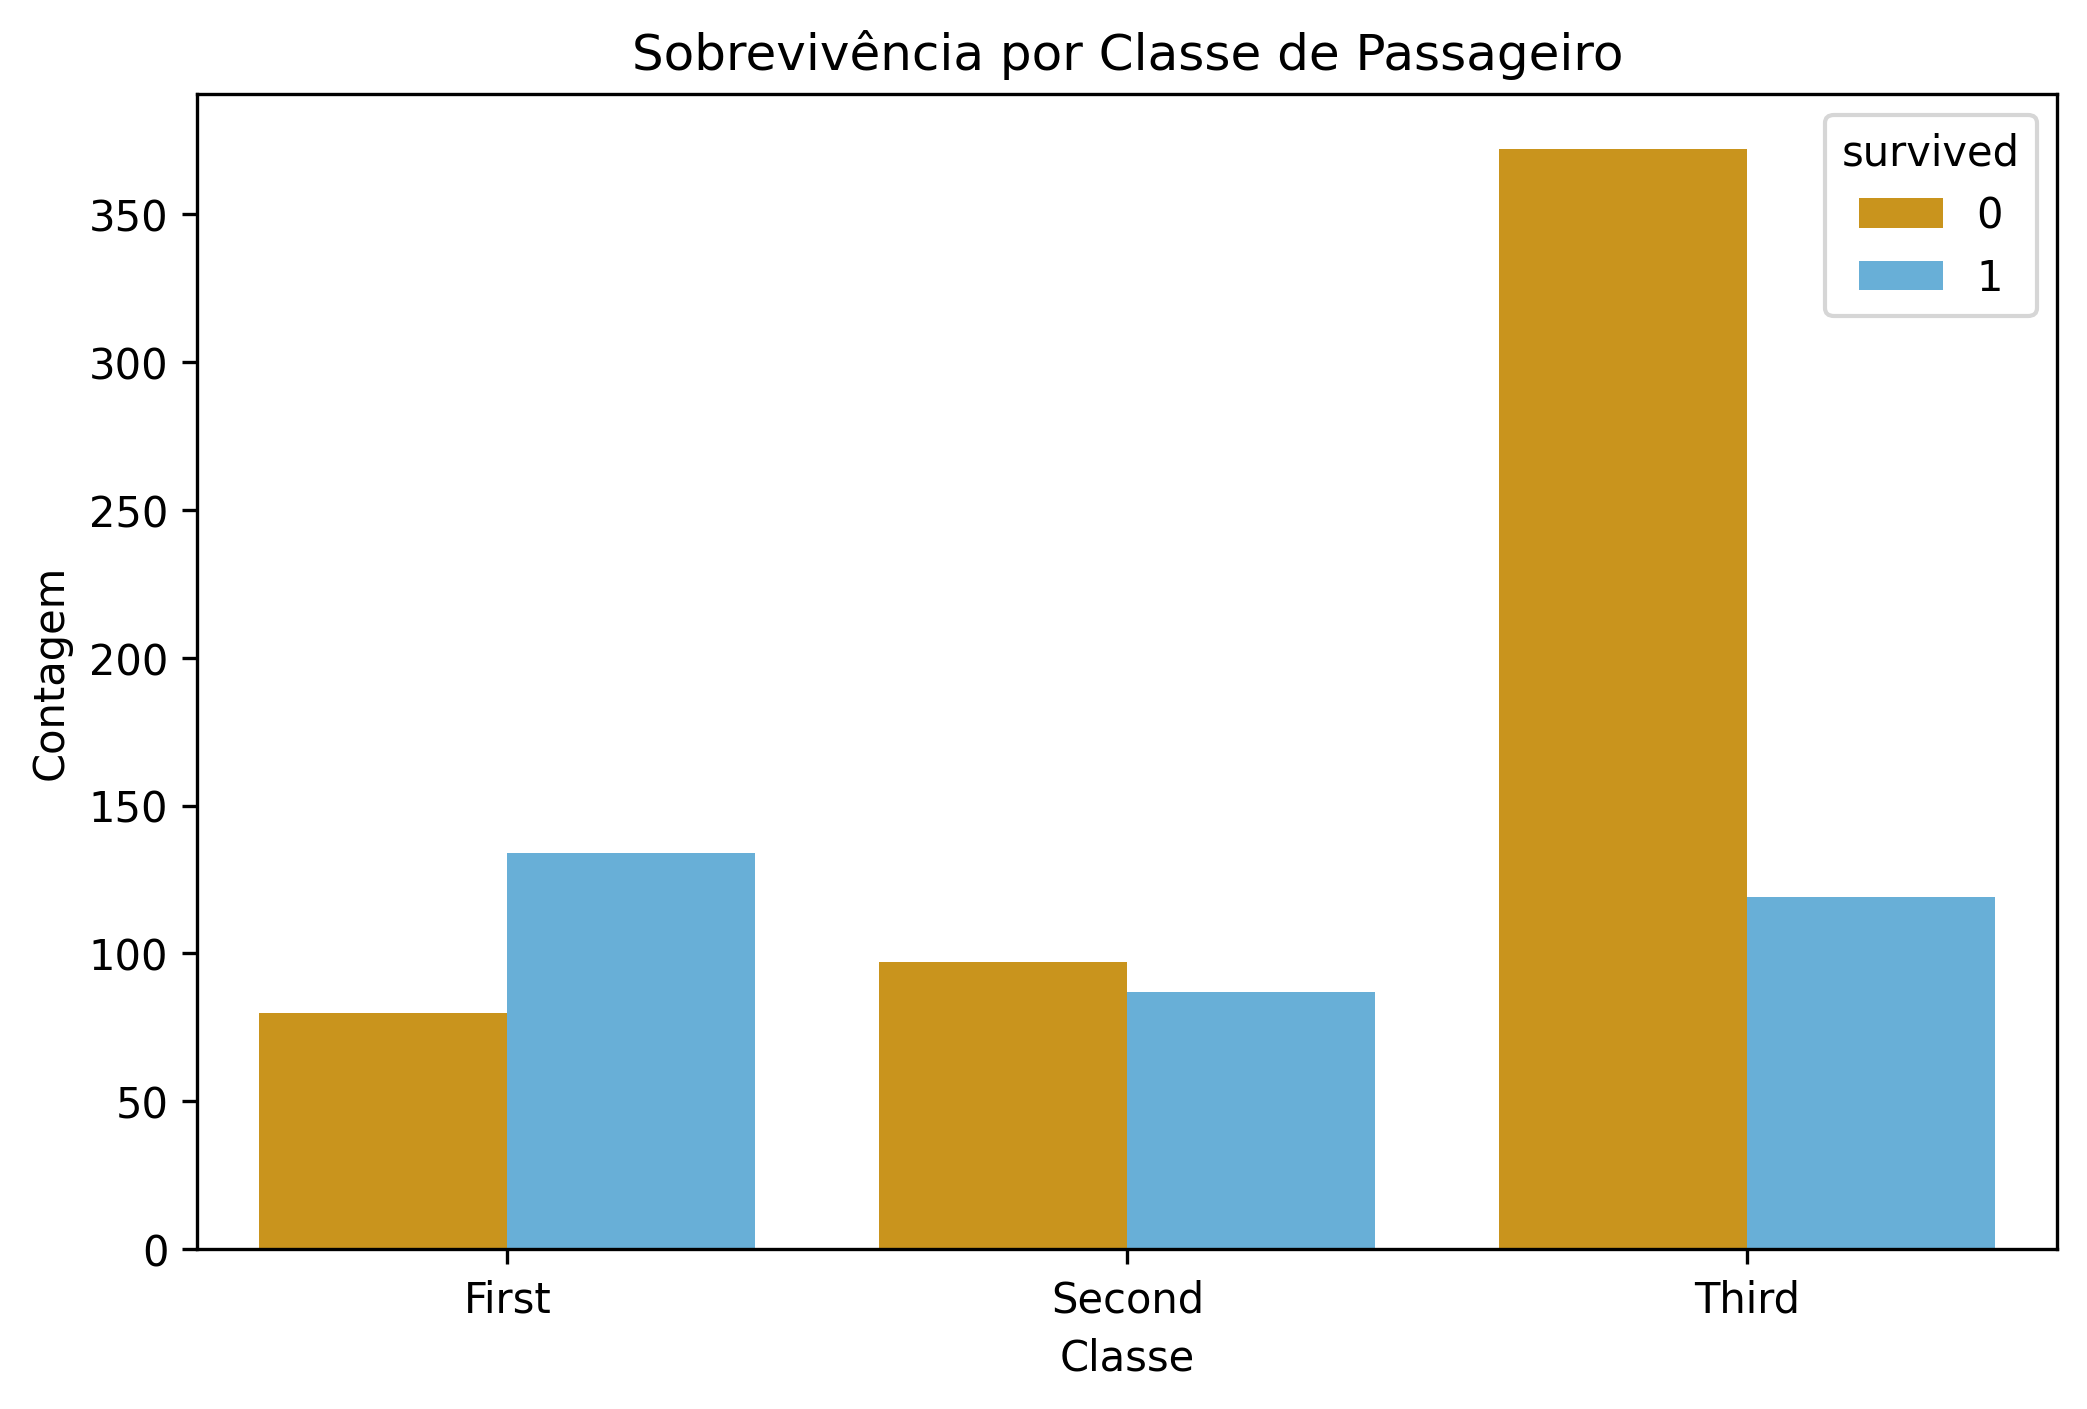
\includegraphics[keepaspectratio]{capitulos/analise_exploratoria_files/figure-pdf/cell-2-output-3.png}}

\subsection{\texorpdfstring{Análise de Dados Contínuos:
\emph{Iris}}{Análise de Dados Contínuos: Iris}}\label{anuxe1lise-de-dados-contuxednuos-iris}

A base \texttt{Iris}, introduzida pelo estatístico \emph{Ronald Fisher}
em 1936, é o exemplo definitivo para o estudo de distribuições contínuas
e análise de correlação entre múltiplas variáveis numéricas (como
comprimento e largura de pétalas e sépalas).

Antes de partirmos para a visualização, a extração de métricas de
posição e dispersão é o passo primário para a compreensão de variáveis
contínuas. No \emph{R}, essa tarefa é comumente realizada através da
função \texttt{summary()}. No \emph{Python}, a biblioteca
\texttt{pandas} fornece o método \texttt{.describe()}, que calcula
instantaneamente a contagem, a média, o desvio padrão e os quartis de
todas as colunas numéricas do \emph{DataFrame}.

Enquanto as métricas descritivas resumem os dados, a exploração de dados
contínuos exige uma abordagem visual para a identificação de padrões
lineares ou de agrupamentos (\emph{clusters}). O gráfico de dispersão
(\emph{scatterplot}) é a ferramenta analítica primária para esse fim. O
\texttt{seaborn} permite estratificar esses pontos facilmente através do
parâmetro \texttt{hue}, colorindo as observações com base em uma
variável categórica, como a espécie da flor.

\begin{Shaded}
\begin{Highlighting}[]
\CommentTok{\# Carregando a base de dados}
\NormalTok{iris }\OperatorTok{=}\NormalTok{ sns.load\_dataset(}\StringTok{\textquotesingle{}iris\textquotesingle{}}\NormalTok{)}

\CommentTok{\# Extração das métricas descritivas (equivalente ao summary do R)}
\BuiltInTok{print}\NormalTok{(}\StringTok{"Resumo Estatístico da Base Iris:}\CharTok{\textbackslash{}n}\StringTok{"}\NormalTok{)}
\BuiltInTok{print}\NormalTok{(iris.describe())}

\CommentTok{\# Configurando e gerando o gráfico de dispersão com Seaborn}
\NormalTok{plt.figure(figsize}\OperatorTok{=}\NormalTok{(}\DecValTok{8}\NormalTok{, }\DecValTok{5}\NormalTok{))}
\NormalTok{sns.scatterplot(}
\NormalTok{    data}\OperatorTok{=}\NormalTok{iris, }
\NormalTok{    x}\OperatorTok{=}\StringTok{\textquotesingle{}petal\_length\textquotesingle{}}\NormalTok{, }
\NormalTok{    y}\OperatorTok{=}\StringTok{\textquotesingle{}petal\_width\textquotesingle{}}\NormalTok{, }
\NormalTok{    hue}\OperatorTok{=}\StringTok{\textquotesingle{}species\textquotesingle{}}\NormalTok{, }
\NormalTok{    palette}\OperatorTok{=}\NormalTok{[}\StringTok{"\#E69F00"}\NormalTok{, }\StringTok{"\#56B4E9"}\NormalTok{, }\StringTok{"\#CC79A7"}\NormalTok{],}
\NormalTok{    s}\OperatorTok{=}\DecValTok{80} \CommentTok{\# Tamanho dos pontos}
\NormalTok{)}
\NormalTok{plt.title(}\StringTok{"Relação entre Comprimento e Largura da Pétala"}\NormalTok{)}
\NormalTok{plt.xlabel(}\StringTok{"Comprimento da Pétala (cm)"}\NormalTok{)}
\NormalTok{plt.ylabel(}\StringTok{"Largura da Pétala (cm)"}\NormalTok{)}
\NormalTok{plt.show()}
\end{Highlighting}
\end{Shaded}

\begin{verbatim}
Resumo Estatístico da Base Iris:

       sepal_length  sepal_width  petal_length  petal_width
count    150.000000   150.000000    150.000000   150.000000
mean       5.843333     3.057333      3.758000     1.199333
std        0.828066     0.435866      1.765298     0.762238
min        4.300000     2.000000      1.000000     0.100000
25%        5.100000     2.800000      1.600000     0.300000
50%        5.800000     3.000000      4.350000     1.300000
75%        6.400000     3.300000      5.100000     1.800000
max        7.900000     4.400000      6.900000     2.500000
\end{verbatim}

\pandocbounded{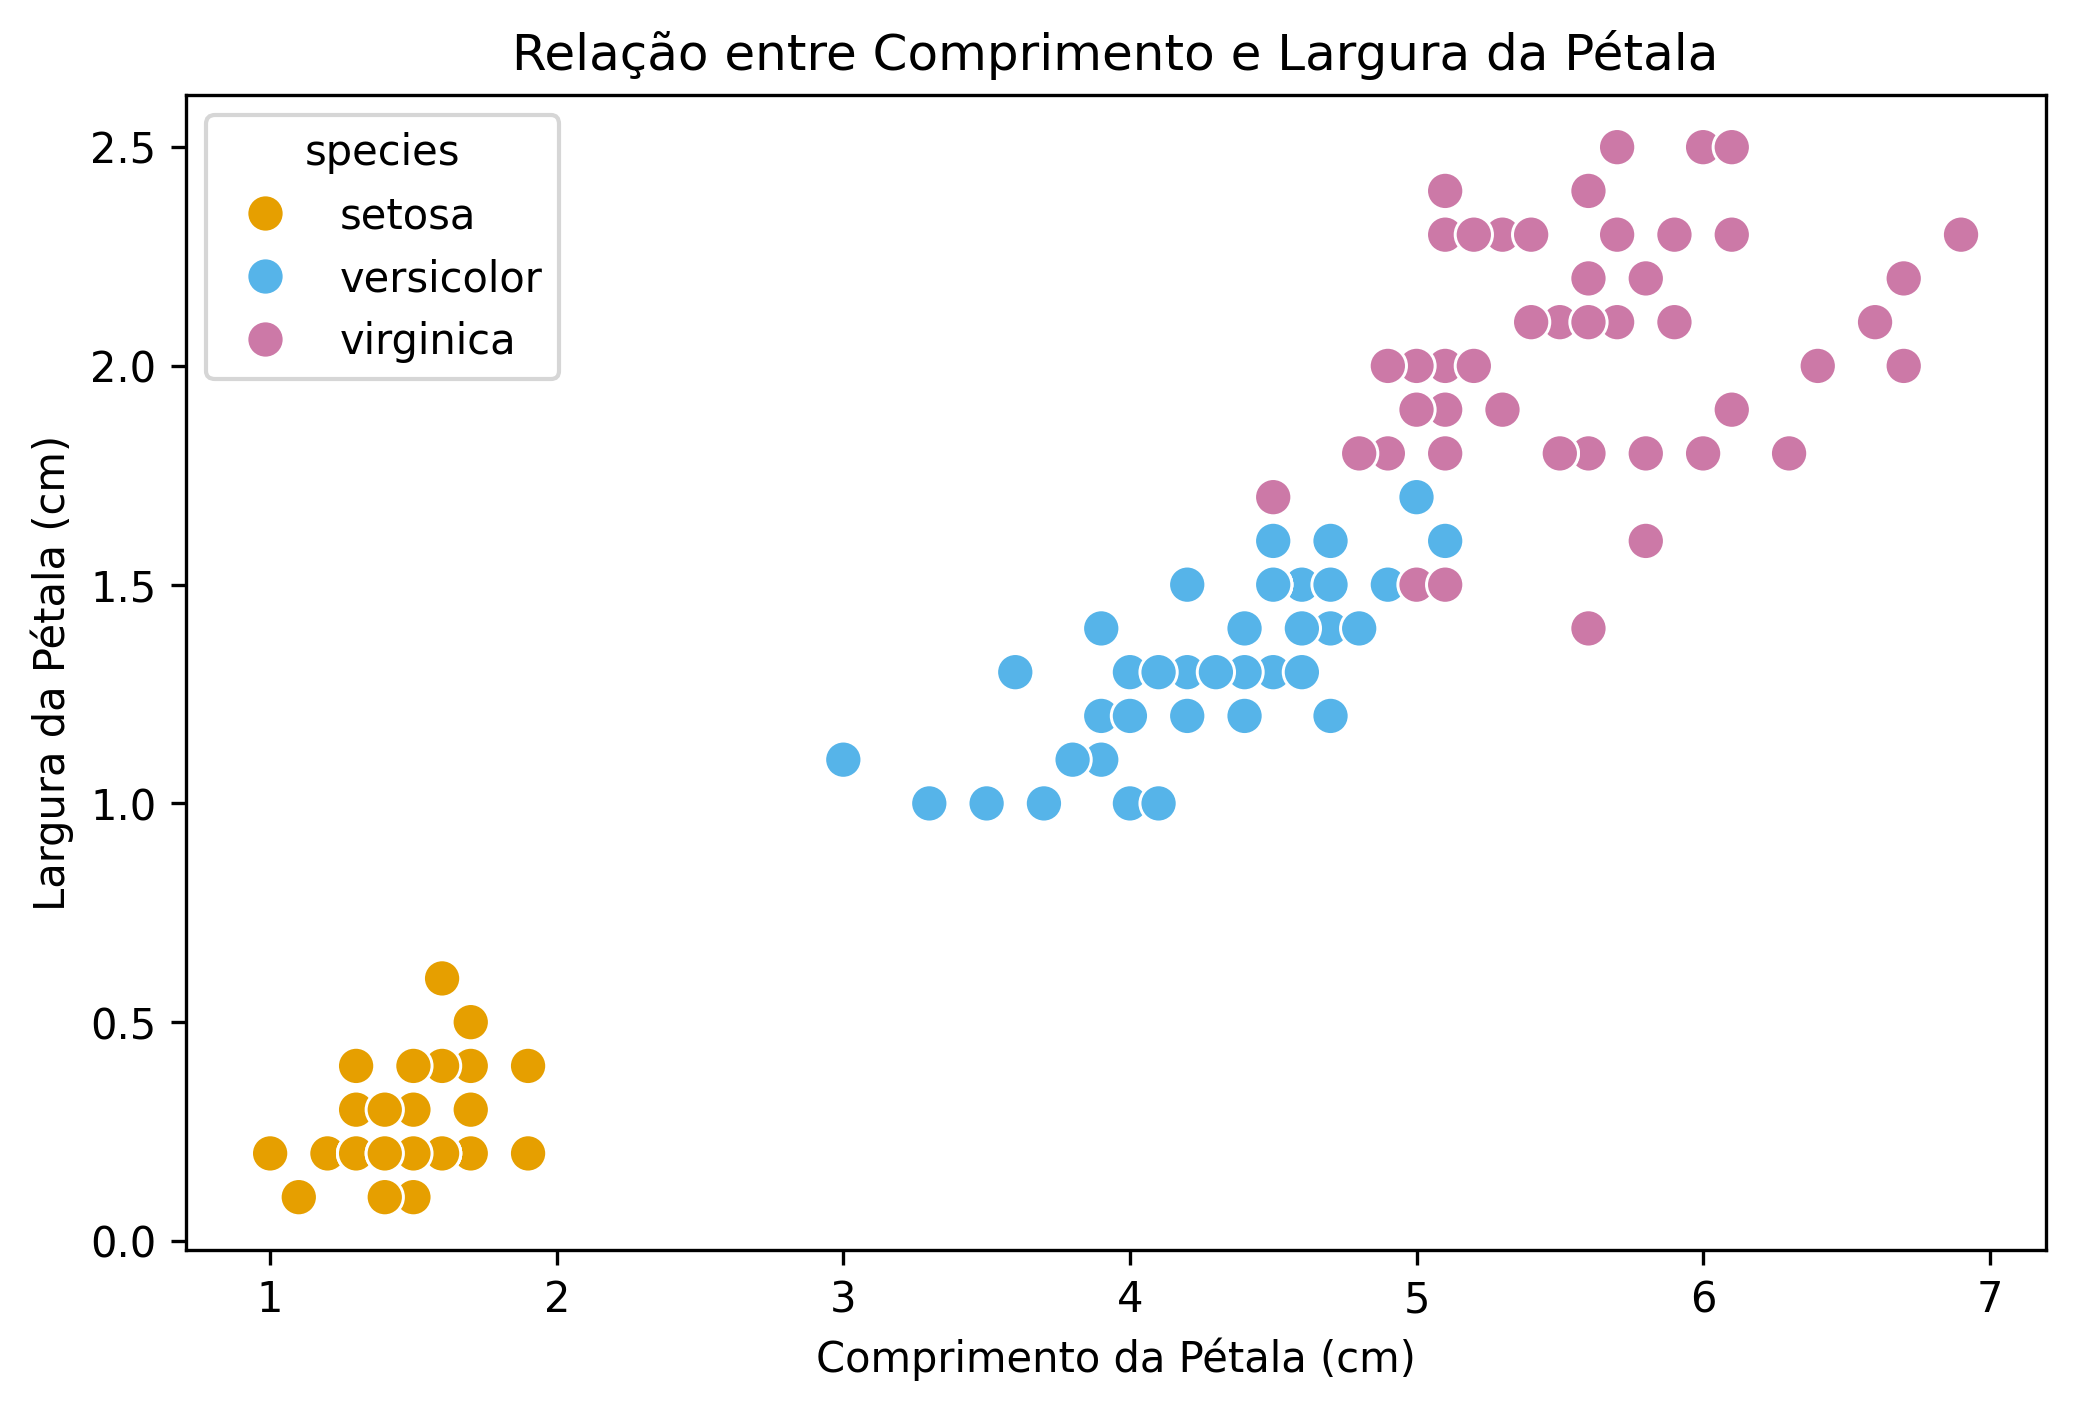
\includegraphics[keepaspectratio]{capitulos/analise_exploratoria_files/figure-pdf/cell-3-output-2.png}}

\bookmarksetup{startatroot}

\chapter{Computação Numérica com
NumPy}\label{computauxe7uxe3o-numuxe9rica-com-numpy}

\begin{center}\rule{0.5\linewidth}{0.5pt}\end{center}

Apesar da versatilidade e da sintaxe amigável, podemos encontrar
problema ao trabalhar com computação matemática em \emph{Python}. Isso
ocorre porque o \emph{Python} não foi concebido originalmente para o
trabalho científico, ao contrário do \emph{R} por exemplo, que já foi
desenvolvida de forma vetorizada, voltada para trabalhar com
Estatística.

É para preencher essa lacuna que surge a biblioteca \texttt{numpy}
(\emph{Numerical Python}). Ela atua como o alicerce do ecossistema de
dados da linguagem, sendo, inclusive, a base matemática oculta que atua
por trás do \texttt{pandas}, do \texttt{matplotlib} e de bibliotecas de
aprendizado de máquina.

\section{A Revolução Vetorial e o
Objeto}\label{a-revoluuxe7uxe3o-vetorial-e-o-objeto}

Como vimos, a principal estrutura de dados do \emph{Python} para
armazenar vetores de dados é a lista (\texttt{list}). As listas são
extremamente flexíveis, permitem armazenar dados de diferentes tipos
nativamente e, até mesmo, armazenar outras listas dentro de uma lista.
Porém, do ponto de vista computacional, essa maleabilidade tem um custo
elevado: as listas não armazenam os dados em si de forma contínua na
memória, mas sim ponteiros para onde as informações estão. Como é de se
imaginar, isso torna o processamento de grandes bases de dados
extremamente custoso computacionalmente falando, já que as iterações
estariam sendo feitas sobre os ponteiros.

A revolução trazida pelo \texttt{numpy} baseia-se na introdução de um
novo objeto fundamental: o \emph{array} multidimensional, conhecido pela
classe \texttt{ndarray} (\emph{n-dimensional array}) (Harris et al.,
2020). Diferentemente das listas, um \texttt{ndarray} exige tipagem
estática, o que significa que todos os elementos em seu interior devem
ser estritamente do mesmo tipo (geralmente numérico). Essa homogeneidade
permite que os dados sejam alocados na memória de forma adjacente,
fazendo com que a eficiência dos cálculos se aproxime bastante a de
linguagens compiladas, como o \emph{C++}, por exemplo.

Para o trabalho estatístico, a maior vantagem do \texttt{ndarray} é
permitir a vetorização. Operações matemáticas aplicadas a um
\emph{array} são executadas em toda a estrutura simultaneamente,
eliminando por completo a necessidade de escrever laços de repetição
manuais (\emph{for} ou \emph{while}).

O bloco de código a seguir ilustra a diferença na sintaxe e no
comportamento ao realizarmos uma soma elemento a elemento entre dois
vetores numéricos usando o \emph{Python} puro e o \texttt{numpy}:

\begin{Shaded}
\begin{Highlighting}[]
\ImportTok{import}\NormalTok{ numpy }\ImportTok{as}\NormalTok{ np}

\CommentTok{\# Soma elemento a elemento com Python puro (Listas)}
\NormalTok{lista\_a }\OperatorTok{=}\NormalTok{ [}\DecValTok{1}\NormalTok{, }\DecValTok{2}\NormalTok{, }\DecValTok{3}\NormalTok{, }\DecValTok{4}\NormalTok{]}
\NormalTok{lista\_b }\OperatorTok{=}\NormalTok{ [}\DecValTok{10}\NormalTok{, }\DecValTok{20}\NormalTok{, }\DecValTok{30}\NormalTok{, }\DecValTok{40}\NormalTok{]}

\CommentTok{\# Exige conhecimento de listas e iteração explícita com a função zip}
\NormalTok{soma\_listas }\OperatorTok{=}\NormalTok{ [a }\OperatorTok{+}\NormalTok{ b }\ControlFlowTok{for}\NormalTok{ a, b }\KeywordTok{in} \BuiltInTok{zip}\NormalTok{(lista\_a, lista\_b)]}
\BuiltInTok{print}\NormalTok{(}\SpecialStringTok{f"Soma com listas nativas: }\SpecialCharTok{\{}\NormalTok{soma\_listas}\SpecialCharTok{\}}\SpecialStringTok{"}\NormalTok{)}

\CommentTok{\# Soma elemento a elemento com NumPy (ndarrays)}
\NormalTok{array\_a }\OperatorTok{=}\NormalTok{ np.array([}\DecValTok{1}\NormalTok{, }\DecValTok{2}\NormalTok{, }\DecValTok{3}\NormalTok{, }\DecValTok{4}\NormalTok{])}
\NormalTok{array\_b }\OperatorTok{=}\NormalTok{ np.array([}\DecValTok{10}\NormalTok{, }\DecValTok{20}\NormalTok{, }\DecValTok{30}\NormalTok{, }\DecValTok{40}\NormalTok{])}

\CommentTok{\# Operação vetorizada direta, parecido com o R}
\NormalTok{soma\_arrays }\OperatorTok{=}\NormalTok{ array\_a }\OperatorTok{+}\NormalTok{ array\_b}
\BuiltInTok{print}\NormalTok{(}\SpecialStringTok{f"Soma com arrays do NumPy:  }\SpecialCharTok{\{}\NormalTok{soma\_arrays}\SpecialCharTok{\}}\SpecialStringTok{"}\NormalTok{)}
\end{Highlighting}
\end{Shaded}

\begin{verbatim}
Soma com listas nativas: [11, 22, 33, 44]
Soma com arrays do NumPy:  [11 22 33 44]
\end{verbatim}

\section{Criação e Formatação de
Matrizes}\label{criauxe7uxe3o-e-formatauxe7uxe3o-de-matrizes}

Na prática, raramente digitamos manualmente os valores de uma matriz.
Neste contexto, o \texttt{numpy} oferece diversas funções geradoras
otimizadas para criar vetores e matrizes (McKinney, 2022).

As funções \texttt{np.zeros()} e \texttt{np.ones()} criam \emph{arrays}
preenchidos exclusivamente por zeros ou uns, respectivamente, bastando
informar a dimensão desejada. Para criar sequências numéricas, o
\texttt{np.arange()} funciona de maneira análoga à função \texttt{seq()}
do \emph{R} ou \texttt{range()} do \emph{Python}, gerando valores com
base em um limite inicial, um limite final e um passo. Já o
\texttt{np.linspace()} é extremamente útil na criação de pontos para
distribuições ou gráficos, pois gera um número exato de valores
linearmente espaçados dentro de um intervalo fechado.

Além da criação, a manipulação da dimensionalidade é uma tarefa
constante preparação dos dados, com a qual todo analista tem que lidar.
Todo \emph{array} do \texttt{numpy} possui o atributo \texttt{.shape},
que retorna uma tupla com o tamanho de cada dimensão, e o atributo
\texttt{.ndim}, que indica o número total de dimensões (1 para vetores,
2 para matrizes, etc.).

Caso seja necessário alterar a estrutura de um conjunto de dados sem
modificar seus valores numéricos originais --- como transformar um vetor
unidimensional de 12 elementos em uma matriz bidimensional de 3 linhas e
4 colunas --- o método \texttt{.reshape()} realiza essa transposição
instantaneamente.

O script a seguir demonstra essas ferramentas em ação:

\begin{Shaded}
\begin{Highlighting}[]
\CommentTok{\# Geração de matrizes básicas}
\CommentTok{\# O parâmetro é uma tupla indicando (linhas, colunas)}
\NormalTok{matriz\_zeros }\OperatorTok{=}\NormalTok{ np.zeros((}\DecValTok{2}\NormalTok{, }\DecValTok{3}\NormalTok{)) }
\BuiltInTok{print}\NormalTok{(}\SpecialStringTok{f"Matriz de Zeros:}\CharTok{\textbackslash{}n}\SpecialCharTok{\{}\NormalTok{matriz\_zeros}\SpecialCharTok{\}}\CharTok{\textbackslash{}n}\SpecialStringTok{"}\NormalTok{)}

\CommentTok{\# Sequências numéricas}
\NormalTok{vetor\_sequencia }\OperatorTok{=}\NormalTok{ np.arange(}\DecValTok{0}\NormalTok{, }\DecValTok{10}\NormalTok{, }\DecValTok{2}\NormalTok{) }\CommentTok{\# De 0 a 10 (exclusivo), passo 2}
\BuiltInTok{print}\NormalTok{(}\SpecialStringTok{f"Sequência com arange: }\SpecialCharTok{\{}\NormalTok{vetor\_sequencia}\SpecialCharTok{\}}\CharTok{\textbackslash{}n}\SpecialStringTok{"}\NormalTok{)}

\NormalTok{vetor\_linear }\OperatorTok{=}\NormalTok{ np.linspace(}\DecValTok{0}\NormalTok{, }\DecValTok{1}\NormalTok{, }\DecValTok{5}\NormalTok{) }\CommentTok{\# 5 valores uniformemente espaçados entre 0 e 1}
\BuiltInTok{print}\NormalTok{(}\SpecialStringTok{f"Sequência com linspace: }\SpecialCharTok{\{}\NormalTok{vetor\_linear}\SpecialCharTok{\}}\CharTok{\textbackslash{}n}\SpecialStringTok{"}\NormalTok{)}

\CommentTok{\# Manipulação de dimensionalidade}
\NormalTok{vetor\_base }\OperatorTok{=}\NormalTok{ np.arange(}\DecValTok{1}\NormalTok{, }\DecValTok{13}\NormalTok{)}
\BuiltInTok{print}\NormalTok{(}\SpecialStringTok{f"Vetor Original (1D): }\SpecialCharTok{\{}\NormalTok{vetor\_base}\SpecialCharTok{\}}\SpecialStringTok{"}\NormalTok{)}
\BuiltInTok{print}\NormalTok{(}\SpecialStringTok{f"Formato: }\SpecialCharTok{\{}\NormalTok{vetor\_base}\SpecialCharTok{.}\NormalTok{shape}\SpecialCharTok{\}}\SpecialStringTok{ | Dimensões: }\SpecialCharTok{\{}\NormalTok{vetor\_base}\SpecialCharTok{.}\NormalTok{ndim}\SpecialCharTok{\}}\CharTok{\textbackslash{}n}\SpecialStringTok{"}\NormalTok{)}

\CommentTok{\# Transformando o vetor 1D em uma matriz 2D (3 linhas, 4 colunas)}
\NormalTok{matriz\_remodelada }\OperatorTok{=}\NormalTok{ vetor\_base.reshape(}\DecValTok{3}\NormalTok{, }\DecValTok{4}\NormalTok{)}
\BuiltInTok{print}\NormalTok{(}\SpecialStringTok{f"Matriz Remodelada (2D):}\CharTok{\textbackslash{}n}\SpecialCharTok{\{}\NormalTok{matriz\_remodelada}\SpecialCharTok{\}}\SpecialStringTok{"}\NormalTok{)}
\BuiltInTok{print}\NormalTok{(}\SpecialStringTok{f"Novo Formato: }\SpecialCharTok{\{}\NormalTok{matriz\_remodelada}\SpecialCharTok{.}\NormalTok{shape}\SpecialCharTok{\}}\SpecialStringTok{ | Dimensões: }\SpecialCharTok{\{}\NormalTok{matriz\_remodelada}\SpecialCharTok{.}\NormalTok{ndim}\SpecialCharTok{\}}\SpecialStringTok{"}\NormalTok{)}
\end{Highlighting}
\end{Shaded}

\begin{verbatim}
Matriz de Zeros:
[[0. 0. 0.]
 [0. 0. 0.]]

Sequência com arange: [0 2 4 6 8]

Sequência com linspace: [0.   0.25 0.5  0.75 1.  ]

Vetor Original (1D): [ 1  2  3  4  5  6  7  8  9 10 11 12]
Formato: (12,) | Dimensões: 1

Matriz Remodelada (2D):
[[ 1  2  3  4]
 [ 5  6  7  8]
 [ 9 10 11 12]]
Novo Formato: (3, 4) | Dimensões: 2
\end{verbatim}

\section{\texorpdfstring{Álgebra, \emph{Broadcasting} e Indexação
Booleana}{Álgebra, Broadcasting e Indexação Booleana}}\label{uxe1lgebra-broadcasting-e-indexauxe7uxe3o-booleana}

A álgebra matricial clássica exige que duas matrizes tenham formatos
compatíveis para realizar operações como soma ou multiplicação. Porém, o
\texttt{numpy} apresenta um recurso computacional extremamente
otimizado, chamado de \emph{Broadcasting} (Harris et al., 2020), que
aumenta consideravelmente essa flexibilidade operacional. Esse recurso
permite que o \emph{Python} alinhe e opere vetores de diferentes
dimensões sem a necessidade de duplicar dados na memória.

Um exemplo clássico do \emph{Broadcasting} é quando multiplicamos um
\emph{array} por um escalar. O escalar é virtualmente ``esticado'' ou
transmitido por toda a dimensão do array, aplicando a operação a cada
elemento individualmente. Isso facilita bastante a padronização de dados
estatísticos (como subtrair a média e dividir pelo desvio padrão de um
vetor).

Além da álgebra vetorizada, a manipulaçãqo de matrizes também requer
métodos eficientes de filtragem. Para tal, o \emph{R} oferece um suporte
nativo da linguagem, que já é vetorizada em sua base. No \emph{Python},
é o \texttt{numpy} que reproduz essa característica, através da
Indexação Booleana (ou Máscara Booleana).

Ao aplicarmos uma condição lógica a um \texttt{ndarray} (por exemplo,
vetor \textgreater{} 5), a biblioteca não avalia a estrutura inteira
como uma única expressão, mas sim elemento a elemento, retornando um
novo \emph{array} contendo valores lógicos (\emph{True} ou
\emph{False}). Ao passarmos essa ``máscara'' dentro dos colchetes do
\emph{array} original, o \texttt{numpy} filtra e retorna exclusivamente
os elementos onde a condição for verdadeira.

O código a seguir demonstra o poder combinado do \emph{Broadcasting} e
das indexações lógicas:

\begin{Shaded}
\begin{Highlighting}[]
\ImportTok{import}\NormalTok{ numpy }\ImportTok{as}\NormalTok{ np}

\CommentTok{\# Criando um array de base para testes}
\NormalTok{dados }\OperatorTok{=}\NormalTok{ np.array([}\DecValTok{12}\NormalTok{, }\DecValTok{15}\NormalTok{, }\DecValTok{22}\NormalTok{, }\DecValTok{9}\NormalTok{, }\DecValTok{31}\NormalTok{, }\DecValTok{18}\NormalTok{, }\DecValTok{4}\NormalTok{])}
\BuiltInTok{print}\NormalTok{(}\SpecialStringTok{f"Vetor original: }\SpecialCharTok{\{}\NormalTok{dados}\SpecialCharTok{\}}\CharTok{\textbackslash{}n}\SpecialStringTok{"}\NormalTok{)}

\CommentTok{\# 1. Aplicação de Broadcasting (Escalar sobre Array)}
\CommentTok{\# Multiplicando todos os elementos por 2 e somando 10}
\NormalTok{dados\_transformados }\OperatorTok{=}\NormalTok{ (dados }\OperatorTok{*} \DecValTok{2}\NormalTok{) }\OperatorTok{+} \DecValTok{10}
\BuiltInTok{print}\NormalTok{(}\SpecialStringTok{f"Broadcasting (dados * 2 + 10): }\SpecialCharTok{\{}\NormalTok{dados\_transformados}\SpecialCharTok{\}}\CharTok{\textbackslash{}n}\SpecialStringTok{"}\NormalTok{)}

\CommentTok{\# 2. Máscara Booleana (Condição Lógica)}
\NormalTok{mascara }\OperatorTok{=}\NormalTok{ dados }\OperatorTok{\textgreater{}} \DecValTok{15}
\BuiltInTok{print}\NormalTok{(}\SpecialStringTok{f"Máscara Lógica (dados \textgreater{} 15): }\SpecialCharTok{\{}\NormalTok{mascara}\SpecialCharTok{\}}\CharTok{\textbackslash{}n}\SpecialStringTok{"}\NormalTok{)}

\CommentTok{\# 3. Indexação Booleana (Filtragem direta)}
\NormalTok{dados\_filtrados }\OperatorTok{=}\NormalTok{ dados[dados }\OperatorTok{\textgreater{}} \DecValTok{15}\NormalTok{]}
\BuiltInTok{print}\NormalTok{(}\SpecialStringTok{f"Vetor filtrado (apenas valores \textgreater{} 15): }\SpecialCharTok{\{}\NormalTok{dados\_filtrados}\SpecialCharTok{\}}\CharTok{\textbackslash{}n}\SpecialStringTok{"}\NormalTok{)}

\CommentTok{\# 4. Indexação com múltiplas condições (uso dos operadores \& e |)}
\CommentTok{\# Filtrando valores pares E maiores que 10}
\CommentTok{\# Obs: É obrigatório o uso de parênteses em múltiplas condições no numpy}
\NormalTok{filtro\_complexo }\OperatorTok{=}\NormalTok{ dados[(dados }\OperatorTok{\textgreater{}} \DecValTok{10}\NormalTok{) }\OperatorTok{\&}\NormalTok{ (dados }\OperatorTok{\%} \DecValTok{2} \OperatorTok{==} \DecValTok{0}\NormalTok{)]}
\BuiltInTok{print}\NormalTok{(}\SpecialStringTok{f"Valores pares maiores que 10: }\SpecialCharTok{\{}\NormalTok{filtro\_complexo}\SpecialCharTok{\}}\SpecialStringTok{"}\NormalTok{)}
\end{Highlighting}
\end{Shaded}

\begin{verbatim}
Vetor original: [12 15 22  9 31 18  4]

Broadcasting (dados * 2 + 10): [34 40 54 28 72 46 18]

Máscara Lógica (dados > 15): [False False  True False  True  True False]

Vetor filtrado (apenas valores > 15): [22 31 18]

Valores pares maiores que 10: [12 22 18]
\end{verbatim}

\section{Funções Estatísticas e Simulação
Aleatória}\label{funuxe7uxf5es-estatuxedsticas-e-simulauxe7uxe3o-aleatuxf3ria}

O último pilar a ser explorado do \texttt{numpy}, talvez onde realmente
consigamos contextualizar bastante o trabalho do Estatístico usando o
\emph{Python}, é a sua capacidade de realizar computação estatística e
gerar números pseudoaleatórios. Para cálculos descritivos, os
\emph{arrays} contam com métodos nativos altamente otimizados (como
\texttt{.mean()}, \texttt{.sum()}, \texttt{.var()} e \texttt{.std()})
que operam em frações de segundo, mesmo em vetores com milhões de
observações (Harris et al., 2020).

Contudo, para o estatístico, o verdadeiro poder da biblioteca está no
submódulo \texttt{np.random}. Ele permite a simulação estocástica a
partir das mais variadas famílias de distribuições de probabilidade
(Normal, Binomial, Poisson, Exponencial, entre outras), sendo a
ferramenta base para simulações de Monte Carlo e reamostragem.

Para demonstrar a confiabilidade computacional do numpy, realizaremos
dois experimentos empíricos clássicos da teoria das probabilidades:

\textbf{1. A Propriedade da Soma da Distribuição de Poisson}

Matematicamente, sabemos que se extrairmos uma amostra aleatória de
tamanho \(n\) de uma população que segue uma distribuição de Poisson com
parâmetro \(\theta\), o somatório dos valores dessa amostra não é apenas
uma acumulação aleatória; o somatório do parâmetro \(\theta\) em uma
amostra de tamanho \(n\) deve ser representado exatamente como
\(n\theta\). Vamos simular uma amostra grande e verificar o valor
empírico contra esse valor teórico esperado.

\textbf{2. Convergência Assintótica (Teorema Central do Limite)}

\emph{O Teorema Central do Limite (TCL)} postula que a distribuição das
médias amostrais de variáveis independentes e identicamente distribuídas
converge assintoticamente para uma distribuição Normal à medida que o
tamanho da amostra (\(n\)) cresce, independentemente da distribuição
original dos dados. Simularemos milhares de amostras extraídas de uma
distribuição estritamente Exponencial (fortemente assimétrica) e
utilizaremos o \texttt{seaborn} (visto no Capítulo 4) para plotar a
densidade das médias, revelando o inconfundível formato de sino.

O script a seguir realiza essas duas simulações:

\begin{Shaded}
\begin{Highlighting}[]
\ImportTok{import}\NormalTok{ numpy }\ImportTok{as}\NormalTok{ np}
\ImportTok{import}\NormalTok{ matplotlib.pyplot }\ImportTok{as}\NormalTok{ plt}
\ImportTok{import}\NormalTok{ seaborn }\ImportTok{as}\NormalTok{ sns}

\CommentTok{\# Fixando a semente para garantir a reprodutibilidade do livro}
\NormalTok{np.random.seed(}\DecValTok{666}\NormalTok{)}

\BuiltInTok{print}\NormalTok{(}\StringTok{"{-}{-}{-} 1. Simulação da Distribuição de Poisson {-}{-}{-}"}\NormalTok{)}
\NormalTok{n\_poisson }\OperatorTok{=} \DecValTok{100000}  \CommentTok{\# Tamanho da amostra}
\NormalTok{theta }\OperatorTok{=} \FloatTok{3.5}         \CommentTok{\# Parâmetro da distribuição}

\CommentTok{\# Gerando o array com a amostra de Poisson}
\NormalTok{amostra\_poisson }\OperatorTok{=}\NormalTok{ np.random.poisson(lam}\OperatorTok{=}\NormalTok{theta, size}\OperatorTok{=}\NormalTok{n\_poisson)}

\CommentTok{\# Calculando o somatório empírico e o teórico (n * theta)}
\NormalTok{soma\_empirica }\OperatorTok{=}\NormalTok{ np.}\BuiltInTok{sum}\NormalTok{(amostra\_poisson)}
\NormalTok{soma\_teorica }\OperatorTok{=}\NormalTok{ n\_poisson }\OperatorTok{*}\NormalTok{ theta}

\BuiltInTok{print}\NormalTok{(}\SpecialStringTok{f"Soma Empírica do array: }\SpecialCharTok{\{}\NormalTok{soma\_empirica}\SpecialCharTok{\}}\SpecialStringTok{"}\NormalTok{)}
\BuiltInTok{print}\NormalTok{(}\SpecialStringTok{f"Valor Teórico Esperado (n * }\CharTok{\textbackslash{}u03b8}\SpecialStringTok{): }\SpecialCharTok{\{}\NormalTok{soma\_teorica}\SpecialCharTok{\}}\CharTok{\textbackslash{}n}\SpecialStringTok{"}\NormalTok{)}


\BuiltInTok{print}\NormalTok{(}\StringTok{"{-}{-}{-} 2. Teorema Central do Limite (Convergência para Normal) {-}{-}{-}"}\NormalTok{)}
\NormalTok{n\_clt }\OperatorTok{=} \DecValTok{500}             \CommentTok{\# Tamanho de cada amostra (n grande)}
\NormalTok{simulacoes }\OperatorTok{=} \DecValTok{10000}      \CommentTok{\# Quantidade de amostras geradas}
\NormalTok{taxa\_lambda }\OperatorTok{=} \FloatTok{2.0}       \CommentTok{\# Parâmetro da distribuição original (Exponencial)}

\CommentTok{\# Simulando 10.000 médias de amostras de tamanho 500}
\CommentTok{\# Criamos uma matriz (10000, 500) e tiramos a média nas linhas (axis=1)}
\NormalTok{matriz\_exponencial }\OperatorTok{=}\NormalTok{ np.random.exponential(scale}\OperatorTok{=}\DecValTok{1}\OperatorTok{/}\NormalTok{taxa\_lambda, size}\OperatorTok{=}\NormalTok{(simulacoes, n\_clt))}
\NormalTok{medias\_amostrais }\OperatorTok{=}\NormalTok{ matriz\_exponencial.mean(axis}\OperatorTok{=}\DecValTok{1}\NormalTok{)}

\BuiltInTok{print}\NormalTok{(}\SpecialStringTok{f"Geradas }\SpecialCharTok{\{}\NormalTok{simulacoes}\SpecialCharTok{\}}\SpecialStringTok{ médias amostrais. Gerando gráfico de densidade..."}\NormalTok{)}

\CommentTok{\# Plotando o resultado para evidenciar a convergência assintótica}
\NormalTok{plt.figure(figsize}\OperatorTok{=}\NormalTok{(}\DecValTok{8}\NormalTok{, }\DecValTok{5}\NormalTok{))}
\NormalTok{sns.histplot(medias\_amostrais, stat}\OperatorTok{=}\StringTok{"density"}\NormalTok{, color}\OperatorTok{=}\StringTok{"\#E69F00"}\NormalTok{, bins}\OperatorTok{=}\DecValTok{60}\NormalTok{, alpha}\OperatorTok{=}\FloatTok{0.7}\NormalTok{)}
\NormalTok{sns.kdeplot(medias\_amostrais, color}\OperatorTok{=}\StringTok{"\#56B4E9"}\NormalTok{, linewidth}\OperatorTok{=}\FloatTok{2.5}\NormalTok{)}
\NormalTok{plt.title(}\SpecialStringTok{f"Teorema Central do Limite (Tamanho da Amostra n = }\SpecialCharTok{\{}\NormalTok{n\_clt}\SpecialCharTok{\}}\SpecialStringTok{)"}\NormalTok{, fontsize}\OperatorTok{=}\DecValTok{14}\NormalTok{)}
\NormalTok{plt.xlabel(}\StringTok{"Médias Amostrais (Distribuição Original: Exponencial)"}\NormalTok{)}
\NormalTok{plt.ylabel(}\StringTok{"Densidade"}\NormalTok{)}
\NormalTok{plt.show()}
\end{Highlighting}
\end{Shaded}

\begin{verbatim}
--- 1. Simulação da Distribuição de Poisson ---
Soma Empírica do array: 350581
Valor Teórico Esperado (n * θ): 350000.0

--- 2. Teorema Central do Limite (Convergência para Normal) ---
Geradas 10000 médias amostrais. Gerando gráfico de densidade...
\end{verbatim}

\pandocbounded{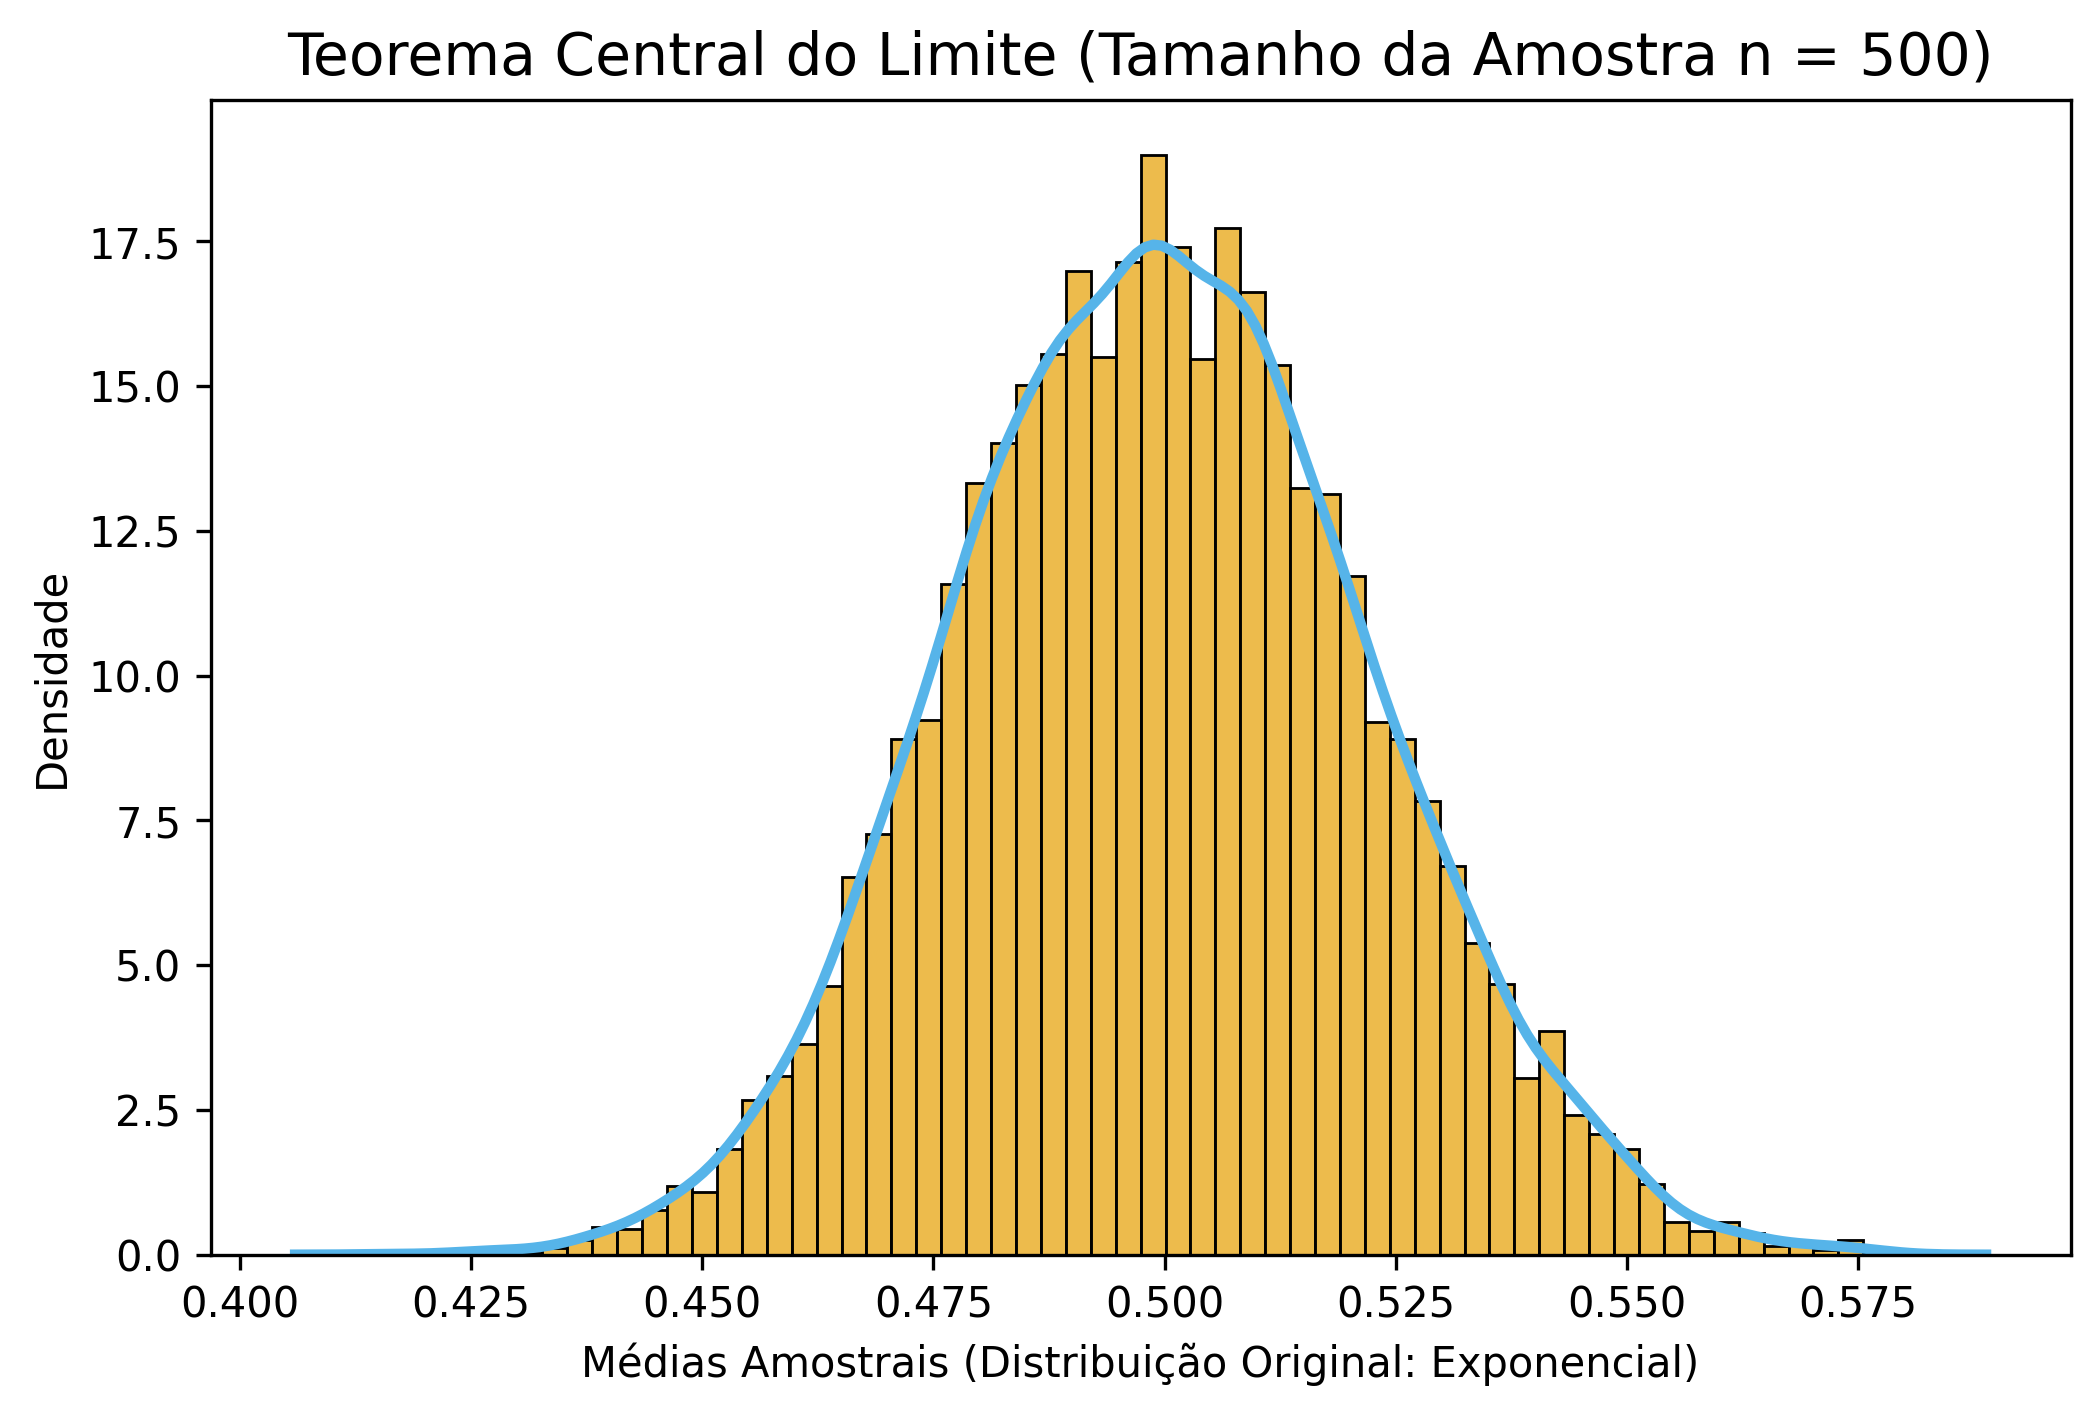
\includegraphics[keepaspectratio]{capitulos/comp_numerica_files/figure-pdf/cell-5-output-2.png}}

\bookmarksetup{startatroot}

\chapter{Web Scraping}\label{web-scraping}

\begin{center}\rule{0.5\linewidth}{0.5pt}\end{center}

Até o momento, o fluxo analítico apresentado pressupôs que os dados já
estivessem estruturados e acessíveis em formatos padronizados (como
arquivos \texttt{CSV}). Contudo, no cenário contemporâneo da Ciência de
Dados, a maior parte das informações geradas diariamente não se encontra
tabularmente organizada, mas sim distribuída em milhões de páginas na
internet. A técnica de acessar, processar e estruturar esses dados de
forma automatizada é conhecida como Web Scraping (raspagem de dados).

\section{\texorpdfstring{Fundamentos da \emph{Web} e Ética na
Extração}{Fundamentos da Web e Ética na Extração}}\label{fundamentos-da-web-e-uxe9tica-na-extrauxe7uxe3o}

Para extrair informações da internet, é essencial compreender a
arquitetura da \emph{web}. Quando acessamos um site, nosso computador (o
cliente) envia uma requisição, através do protocolo \emph{HTTP}
(\emph{Hypertext Transfer Protocol}) para um computador remoto (o
servidor). Na raspagem de dados, a requisição mais comum é o método
\texttt{GET}, utilizado para solicitar a leitura de uma página
(Mitchell, 2018).

Se a requisição for bem-sucedida, o servidor retorna um documento de
texto escrito em \emph{HTML} (\emph{HyperText Markup Language}). O
entendimento da estrutura dos códigos \emph{HTML} sobre os quais as
páginas da \emph{web} são construídas é exatamente o que nos permite
realizar o processo de raspagem de dados.

O \emph{HTML} não é uma linguagem de programação, mas uma linguagem de
marcação, que organiza o conteúdo através de etiquetas (\emph{tags}),
como \texttt{\textless{}p\textgreater{}} para parágrafos,
\texttt{\textless{}h1\textgreater{}} para títulos e
\texttt{\textless{}table\textgreater{}} para tabelas. Esse documento é
estruturado de forma hierárquica, formando uma árvore de elementos
conhecida como \emph{DOM}\footnote{O \emph{DOM} (\emph{Document Object
  Model}) é uma interface de programação que representa o documento
  \emph{HTML} como uma árvore lógica. Ele permite que linguagens de
  programação, como o \emph{Python} ou o \emph{JavaScript}, naveguem,
  acessem e modifiquem o conteúdo, a estrutura e o estilo da página
  \emph{web}.}. É através dos atributos dessas tags (especialmente
\texttt{class} e \texttt{id}) que os algoritmos de scraping conseguem
localizar exatamente qual pedaço de texto ou número deve ser extraído.

Dessa forma, as requisições são guiadas justamente por essas \emph{tags}
que servem como um ``mapa'' da \emph{internet}. Elas nos permitem
generalizar os códigos e buscar, teoricamente, de forma ilimitada pela
web, uma vez que não precisamos conhecer exatamente os textos e seus
caracteres para saber em que local da página buscar, necessitamos apenas
saber qual o local mais provável de se encontrar um conteúdo dentro da
estrutura \emph{HTML}.

\subsection{Ética e Boas Práticas na
Raspagem}\label{uxe9tica-e-boas-pruxe1ticas-na-raspagem}

A raspagem de dados apresenta desafios que vão muito além da capacidade
computacional e da abrangência lógica do código. Um número muito alto de
requisições pode sobrecarregar o servidor alvo, podendo até mesmo
levá-lo a cair, o que configura um ataque de negação de serviço (DDoS)
acidental. Para garantir uma conduta ética, o analista de dados deve
respeitar três pilares fundamentais (Mitchell, 2018):

\begin{itemize}
\item
  Inspeção do arquivo \texttt{robots.txt}: Antes de raspar um domínio,
  deve-se verificar este arquivo público, que contém as diretrizes do
  administrador sobre quais páginas podem ou não ser acessadas por robôs
  (acessível via (nome\_do\_site.com/robots.txt). Por exemplo, se quiser
  raspar dados da \emph{Gov}, deve acessar
  \href{https://www.gov.br/robots.txt}{gov.br/robots.txt}.
\item
  Identificação do \emph{User-Agent}: Por padrão, a biblioteca de
  requisições do Python se identifica como um robô genérico. É
  recomendável alterar o \emph{User-Agent} no cabeçalho da requisição
  para um identificador real (como o de um navegador comum) e, em
  projetos acadêmicos ou comerciais, fornecer um contato válido para o
  administrador do servidor.
\item
  Implementação de \emph{Delays}: O código deve incluir pausas
  intencionais (usando a função \texttt{time.sleep()}) entre as
  requisições, simulando a velocidade de leitura de um ser humano e
  preservando a largura de banda do servidor acessado.
\end{itemize}

\section{O Ecossistema de Raspagem
Estática}\label{o-ecossistema-de-raspagem-estuxe1tica}

Uma vez entendidas as questões éticas da raspagem de dados e estruturais
da \emph{web}, podemos partir para a operacionalização da coleta de
dados. Primeiramente, veremos o caso das páginas cujo conteúdo
\emph{HTML} é entregue, em sua totalidade, logo na requisição inicial.
Nesse caso, dizemos que a extração está sendo feita sobre páginas
estáticas.

O \emph{Python} conta com duas bibliotecas clássicas para a raspagem
estática: a \texttt{requests} e a \texttt{BeautifulSoup}. A biblioteca
\texttt{requests} é responsável por gerenciar a comunicação \emph{HTTP},
nos permitindo baixar os conteúdos de uma página através de comandos
simples e diretos. Um aspecto crucial ao utilizar essa ferramenta é a
validação do código de status da resposta (\emph{status code}). Um
código \texttt{200} indica que a requisição foi bem-sucedida, enquanto
códigos na casa dos \texttt{400} (como o famoso \texttt{404\ Not\ Found}
ou \texttt{403\ Forbidden}) sinalizam, respectivamente, que a página não
existe ou que o servidor bloqueou o acesso, possivelmente identificando
a automação (Mitchell, 2018).

Uma vez que o código \emph{HTML} bruto é capturado com sucesso, ele é
armazenado no computador apenas como uma longa e contínua cadeia de
texto (\emph{string}). Analisar dados diretamente desse formato seria
extremamente comlplicado e suscetível a erros. É neste contexto que a
biblioteca \texttt{BeautifulSoup} (importada do pacote \texttt{bs4}) se
faz necessária.

Ela atua como um ``parseador'' (\emph{parser}), que analisa o texto
bruto e o converte na árvore hierárquica do \emph{DOM}, discutida na
seção anterior. Ao transformar a \emph{string} estática em um objeto
estruturado e navegável, o \texttt{BeautifulSoup} disponibiliza métodos
otimizados para que possamos buscar dados de forma cirúrgica, utilizando
os nomes das \emph{tags} e seus respectivos atributos.

\section{Navegação e Extração de Elementos (Conteúdo
Estático)}\label{navegauxe7uxe3o-e-extrauxe7uxe3o-de-elementos-conteuxfado-estuxe1tico}

Com a página da \emph{web} ``traduzida'' através do
\texttt{BeautifulSoup}, o conteúdo que antes era confuso agora é
estruturado de maneira hierárquica e perfeitamente mapeada. Neste
contexto, nosso desafio passa a ser a localização exata da informação
desejada dentro dessa árvore de elementos (\emph{tags}).

Para navegar por essa estrutura, a biblioteca fornece diversos métodos,
sendo os mais proeminentes o \texttt{find()} e o \texttt{find\_all()}. O
método \texttt{find()} percorre o documento e retorna a primeira
ocorrência de uma \emph{tag} específica que satisfaça os critérios
definidos. Já o \texttt{find\_all()} varre toda a página e retorna uma
coleção (uma lista estruturada) contendo todos os elementos que
correspondam a busca.

Além da busca genérica pelo nome da \emph{tag} (como procurar por todos
os parágrafos \texttt{\textless{}p\textgreater{}}), podemos afunilar a
filtragem através dos atributos da \emph{tag}, especialmente as classes,
utilizando o parâmetro \texttt{class\_} (com um \emph{underline} no
final, para não conflitar com a palavra reservada do \emph{Python}).
Caso o analista possua familiaridade com desenvolvimento \emph{web} (um
dos grandes diferenciais que um analista pode ter no contexto da
raspagem de dados), o método \texttt{select()} permite o uso de
seletores \emph{CSS} diretos, oferecendo uma sintaxe ainda mais concisa
e aumentando as possibilidades de caminhos para as buscas.

Uma vez que o elemento correto é isolado, a extração da informação útil
exige a separação entre o dado e o código \emph{HTML}. O texto visível
aos usuários pode ser extraído acessando a propriedade \texttt{.text} do
objeto. Já quando o objetivo é coletar \emph{links} ou caminhos de
arquivos, a informação desejada não se encontra no texto livre, mas
embutida dentro da própria \emph{tag} (no atributo \texttt{href}), sendo
necessário extraí-la utilizando o método
\texttt{.get(\textquotesingle{}href\textquotesingle{})}.

O \emph{script} a seguir ilustra a aplicação prática desses conceitos
utilizando um documento \emph{HTML} simulado. Essa abordagem garante a
reprodutibilidade metodológica do exemplo, eliminando a dependência de
conexão com servidores externos.

\begin{Shaded}
\begin{Highlighting}[]
\ImportTok{from}\NormalTok{ bs4 }\ImportTok{import}\NormalTok{ BeautifulSoup}

\CommentTok{\# Simulando o HTML estático de uma página estruturada}
\NormalTok{html\_simulado }\OperatorTok{=} \StringTok{"""}
\StringTok{\textless{}html\textgreater{}}
\StringTok{  \textless{}body\textgreater{}}
\StringTok{    \textless{}h1 class="titulo{-}principal"\textgreater{}Estatísticas Demográficas\textless{}/h1\textgreater{}}
\StringTok{    \textless{}p class="resumo"\textgreater{}Este é um resumo dos dados do censo.\textless{}/p\textgreater{}}
\StringTok{    \textless{}div id="dados{-}estatisticos"\textgreater{}}
\StringTok{      \textless{}a href="https://exemplo.com/tabela\_norte.csv" }
\StringTok{      class="link{-}dados"\textgreater{}Dados Região Norte\textless{}/a\textgreater{}}
\StringTok{      \textless{}a href="https://exemplo.com/tabela\_sul.csv" }
\StringTok{      class="link{-}dados"\textgreater{}Dados Região Sul\textless{}/a\textgreater{}}
\StringTok{    \textless{}/div\textgreater{}}
\StringTok{  \textless{}/body\textgreater{}}
\StringTok{\textless{}/html\textgreater{}}
\StringTok{"""}

\CommentTok{\# Instanciando o parser para criar a árvore DOM}
\NormalTok{sopa }\OperatorTok{=}\NormalTok{ BeautifulSoup(html\_simulado, }\StringTok{\textquotesingle{}html.parser\textquotesingle{}}\NormalTok{)}

\CommentTok{\# Usando find() para extrair o texto de uma classe específica}
\NormalTok{titulo }\OperatorTok{=}\NormalTok{ sopa.find(}\StringTok{\textquotesingle{}h1\textquotesingle{}}\NormalTok{, class\_}\OperatorTok{=}\StringTok{\textquotesingle{}titulo{-}principal\textquotesingle{}}\NormalTok{).text}
\BuiltInTok{print}\NormalTok{(}\SpecialStringTok{f"Título da Página: }\SpecialCharTok{\{}\NormalTok{titulo}\SpecialCharTok{\}}\CharTok{\textbackslash{}n}\SpecialStringTok{"}\NormalTok{)}

\CommentTok{\# Usando find\_all() e iterando para extrair e formatar múltiplos links}
\NormalTok{tags\_link }\OperatorTok{=}\NormalTok{ sopa.find\_all(}\StringTok{\textquotesingle{}a\textquotesingle{}}\NormalTok{, class\_}\OperatorTok{=}\StringTok{\textquotesingle{}link{-}dados\textquotesingle{}}\NormalTok{)}

\BuiltInTok{print}\NormalTok{(}\StringTok{"Arquivos Disponíveis para Download:"}\NormalTok{)}
\ControlFlowTok{for}\NormalTok{ tag }\KeywordTok{in}\NormalTok{ tags\_link:}
\NormalTok{    texto\_link }\OperatorTok{=}\NormalTok{ tag.text          }\CommentTok{\# Extrai o texto visível}
\NormalTok{    url }\OperatorTok{=}\NormalTok{ tag.get(}\StringTok{\textquotesingle{}href\textquotesingle{}}\NormalTok{)          }\CommentTok{\# Extrai o link oculto no atributo}
    \BuiltInTok{print}\NormalTok{(}\SpecialStringTok{f"{-} }\SpecialCharTok{\{}\NormalTok{texto\_link}\SpecialCharTok{\}}\SpecialStringTok{: }\SpecialCharTok{\{}\NormalTok{url}\SpecialCharTok{\}}\SpecialStringTok{"}\NormalTok{)}
\end{Highlighting}
\end{Shaded}

\begin{verbatim}
Título da Página: Estatísticas Demográficas

Arquivos Disponíveis para Download:
- Dados Região Norte: https://exemplo.com/tabela_norte.csv
- Dados Região Sul: https://exemplo.com/tabela_sul.csv
\end{verbatim}

\section{\texorpdfstring{Raspagem de Estruturas Tabulares (Integração
com
\texttt{Pandas})}{Raspagem de Estruturas Tabulares (Integração com Pandas)}}\label{raspagem-de-estruturas-tabulares-integrauxe7uxe3o-com-pandas}

Embora os métodos \texttt{find()} e \texttt{find\_all()} do
\texttt{BeautifulSoup} sejam suficientes para extrair qualquer elemento
isolado de uma página, extrair uma estrutura tabular completa (a
\emph{tag} \texttt{\textless{}table\textgreater{}}) elemento por
elemento seria um processo redundante e propenso a erros. Para isso, o
\emph{Python} oferece uma ponte direta o \emph{HTML} tabular e a
estrutura de um \texttt{DataFrame}, através da biblioteca
\texttt{pandas}, da qual já falamos anteriormente.

Neste contexto, destaca-se a função \texttt{pd.read\_html()}, que
automatiza o processo como um todo: ao receber um trecho de código
\emph{HTML}, ela localiza internamente todas as \emph{tags}
\texttt{\textless{}table\textgreater{}} presentes, interpreta suas
linhas (\texttt{\textless{}td\textgreater{}}), e devolve uma lista de
\texttt{DataFrames} prontos para uso - um para cada tabela encontrada no
documento (McKinney, 2022).

É importante destacarque, por razões de segurança, em versões mais
recentes do \texttt{pandas}a função não aceita mais \emph{strings} de
\emph{HTML} diretamente, exigindo que o texto seja envolvido pela classe
\texttt{StringIO} do módulo \texttt{io}, nativo do \emph{Python},
simulando um arquivo em memória.Esse mesmo mecanismo se aplica quando o
\emph{HTML} já foi previamente capturado por uma requisição
\texttt{requests}, sendo a prática recomendada em qualquer cenário de
raspagem real.

O script a seguir demonstra esse fluxo completo, partindo de uma tabela
HTML simulada até a obtenção de um DataFrame estruturado, pronto para as
etapas de tratamento e análise discutidas no Capítulo 4.

\begin{Shaded}
\begin{Highlighting}[]
\ImportTok{import}\NormalTok{ pandas }\ImportTok{as}\NormalTok{ pd}
\ImportTok{from}\NormalTok{ io }\ImportTok{import}\NormalTok{ StringIO}

\CommentTok{\# Simulando uma tabela HTML, como a que poderia ser retornada por uma requisição}
\NormalTok{html\_tabela }\OperatorTok{=} \StringTok{"""}
\StringTok{\textless{}table\textgreater{}}
\StringTok{  \textless{}caption\textgreater{}Indicadores Regionais\textless{}/caption\textgreater{}}
\StringTok{  \textless{}tr\textgreater{}}
\StringTok{    \textless{}th\textgreater{}Região\textless{}/th\textgreater{}}
\StringTok{    \textless{}th\textgreater{}População\textless{}/th\textgreater{}}
\StringTok{    \textless{}th\textgreater{}PIB (em bilhões)\textless{}/th\textgreater{}}
\StringTok{  \textless{}/tr\textgreater{}}
\StringTok{  \textless{}tr\textgreater{}}
\StringTok{    \textless{}td\textgreater{}Norte\textless{}/td\textgreater{}}
\StringTok{    \textless{}td\textgreater{}18000000\textless{}/td\textgreater{}}
\StringTok{    \textless{}td\textgreater{}250\textless{}/td\textgreater{}}
\StringTok{  \textless{}/tr\textgreater{}}
\StringTok{  \textless{}tr\textgreater{}}
\StringTok{    \textless{}td\textgreater{}Sul\textless{}/td\textgreater{}}
\StringTok{    \textless{}td\textgreater{}30000000\textless{}/td\textgreater{}}
\StringTok{    \textless{}td\textgreater{}800\textless{}/td\textgreater{}}
\StringTok{  \textless{}/tr\textgreater{}}
\StringTok{\textless{}/table\textgreater{}}
\StringTok{"""}

\CommentTok{\# read\_html() exige que a string seja envolvida por StringIO}
\NormalTok{tabelas\_encontradas }\OperatorTok{=}\NormalTok{ pd.read\_html(StringIO(html\_tabela))}

\CommentTok{\# A função retorna uma lista de DataFrames (uma por tabela na página)}
\NormalTok{df\_indicadores }\OperatorTok{=}\NormalTok{ tabelas\_encontradas[}\DecValTok{0}\NormalTok{]}

\BuiltInTok{print}\NormalTok{(}\SpecialStringTok{f"Número de tabelas encontradas: }\SpecialCharTok{\{}\BuiltInTok{len}\NormalTok{(tabelas\_encontradas)}\SpecialCharTok{\}}\CharTok{\textbackslash{}n}\SpecialStringTok{"}\NormalTok{)}
\BuiltInTok{print}\NormalTok{(df\_indicadores)}
\end{Highlighting}
\end{Shaded}

\begin{verbatim}
Número de tabelas encontradas: 1

  Região  População  PIB (em bilhões)
0  Norte   18000000               250
1    Sul   30000000               800
\end{verbatim}

Como resultado, obtemos diretamente um \texttt{DataFrame} com tipagem já
inferida (valores numéricos reconhecidos como tais), eliminando por
completo a necessidade de laços de repetição manuais para percorrer
células --- o ``pulo do gato'' analítico mencionado anteriormente. A
partir deste ponto, o `df\_indicadores' já pode ser submetido a qualquer
uma das ferramentas de \emph{Data Wrangling} apresentadas no Capítulo 4,
como \texttt{.describe()}, \texttt{dropna()} ou \texttt{merge()} com
outras bases.

Vale ressaltar que essa abordagem tem uma limitação natural: ela
funciona apenas quando a informação já está de fato estruturada em uma
\emph{tag} \texttt{\textless{}table\textgreater{}} no \emph{HTML.}
Muitas páginas modernas simulam visualmente uma tabela usando
\texttt{\textless{}div\textgreater{}s} estilizados via \emph{CSS}, caso
em que a extração exige o uso combinado de \texttt{find\_all()} ---
técnica que retomaremos no estudo de caso da seção 6.6.

\section{Raspagem Dinâmica e Automação com
Selenium}\label{raspagem-dinuxe2mica-e-automauxe7uxe3o-com-selenium}

As técnicas apresentadas nas seções anteriores partem de uma premissa
importante: o conteúdo relevante já está presente no HTML devolvido pela
requisição inicial. Essa premissa, no entanto, não se sustenta para uma
parcela crescente da web moderna. Em muitas aplicações, o
\texttt{requests} retorna apenas um esqueleto HTML praticamente vazio,
enquanto o conteúdo real (tabelas, listas, resultados de busca) é
inserido dinamicamente na página por código \emph{JavaScript}, executado
somente depois que um navegador carrega e interpreta a página por
completo.

Como o \texttt{BeautifulSoup} não executa \emph{JavaScript} --- ele
apenas interpreta o texto estático que recebe ---, essas páginas exigem
uma abordagem estrutural diferente: em vez de simular uma requisição, é
necessário automatizar um navegador real. É exatamente essa a função da
biblioteca \texttt{Selenium}, originalmente concebida para testes
automatizados de software, mas amplamente adotada pela comunidade de
dados como solução para raspagem dinâmica (Mitchell, 2018).

\subsection{Configuração do
Webdriver}\label{configurauxe7uxe3o-do-webdriver}

O \texttt{Selenium} opera controlando um \emph{webdriver}: um executável
que atua como intermediário entre o código Python e um navegador
instalado na máquina (como o Google Chrome). Em versões mais antigas da
biblioteca, era necessário baixar manualmente o executável
correspondente à versão exata do navegador instalado --- um processo
frágil e propenso a quebras a cada atualização. Desde a versão 4.6, o
\texttt{Selenium} incorpora o \emph{Selenium Manager} (Selenium Project,
2026), um mecanismo interno que detecta automaticamente a versão do
navegador instalado e baixa o \emph{driver} compatível, dispensando essa
configuração manual.

\begin{Shaded}
\begin{Highlighting}[]
\ImportTok{from}\NormalTok{ selenium }\ImportTok{import}\NormalTok{ webdriver}
\ImportTok{from}\NormalTok{ selenium.webdriver.chrome.options }\ImportTok{import}\NormalTok{ Options}

\CommentTok{\# Configurando opções do navegador}
\NormalTok{opcoes }\OperatorTok{=}\NormalTok{ Options()}
\NormalTok{opcoes.add\_argument(}\StringTok{"{-}{-}headless"}\NormalTok{)  }\CommentTok{\# Executa sem abrir uma janela visível}

\CommentTok{\# O Selenium Manager cuida automaticamente do driver compatível}
\NormalTok{navegador }\OperatorTok{=}\NormalTok{ webdriver.Chrome(options}\OperatorTok{=}\NormalTok{opcoes)}

\NormalTok{navegador.get(}\StringTok{"https://www.selenium.dev/selenium/web/web{-}form.html"}\NormalTok{)}
\BuiltInTok{print}\NormalTok{(navegador.title)}

\NormalTok{navegador.quit()  }\CommentTok{\# Encerra o processo do navegador}
\end{Highlighting}
\end{Shaded}

O parâmetro \texttt{-\/-headless} merece destaque: ele instrui o
navegador a operar em segundo plano, sem renderizar uma interface
gráfica visível. Essa é a configuração padrão para scripts de raspagem
em produção, já que reduz o consumo de recursos computacionais.

\subsection{Interação com a
Página}\label{interauxe7uxe3o-com-a-puxe1gina}

Diferentemente do \texttt{BeautifulSoup}, que apenas lê uma
``fotografia'' estática do \emph{HTML}, o \texttt{Selenium} permite
simular ações humanas dentro do navegador controlado. Os métodos mais
utilizados para localizar elementos são agrupados na classe \texttt{By},
que oferece estratégias de busca (por \texttt{ID}, por
\texttt{CSS\_SELECTOR}, por \texttt{XPATH}, entre outras). Uma vez
localizado, o elemento pode ser manipulado através de métodos como
\texttt{.click()}, para simular um clique, e \texttt{.send\_keys()},
para preencher campos de formulário.

\begin{Shaded}
\begin{Highlighting}[]
\ImportTok{from}\NormalTok{ selenium.webdriver.common.by }\ImportTok{import}\NormalTok{ By}

\CommentTok{\# Localizando um campo de texto pelo nome e preenchendo{-}o}
\NormalTok{campo\_texto }\OperatorTok{=}\NormalTok{ navegador.find\_element(By.NAME, }\StringTok{"my{-}text"}\NormalTok{)}
\NormalTok{campo\_texto.send\_keys(}\StringTok{"Estatística com Python"}\NormalTok{)}

\CommentTok{\# Localizando e clicando no botão de envio}
\NormalTok{botao\_envio }\OperatorTok{=}\NormalTok{ navegador.find\_element(By.CSS\_SELECTOR, }\StringTok{"button[type=\textquotesingle{}submit\textquotesingle{}]"}\NormalTok{)}
\NormalTok{botao\_envio.click()}
\end{Highlighting}
\end{Shaded}

\subsection{Espera Explícita e
Implícita}\label{espera-expluxedcita-e-impluxedcita}

Talvez o desafio mais característico da raspagem dinâmica seja o
problema da sincronização: o código \emph{Python} é executado em
milissegundos, mas o carregamento de conteúdo via JavaScript pode levar
segundos, dependendo da conexão e do servidor. Tentar extrair um
elemento antes que ele tenha sido efetivamente renderizado resulta no
erro \texttt{NoSuchElementException}.

Para lidar com essa assincronia, o Selenium oferece dois mecanismos de
espera. A espera implícita, configurada uma única vez com
\texttt{navegador.implicitly\_wait(segundos)}, instrui o driver a
aguardar automaticamente, por um tempo máximo definido, antes de lançar
um erro em qualquer tentativa de busca de elemento. Já a espera
explícita, através da classe \texttt{WebDriverWait}, é uma abordagem
mais precisa e recomendada em cenários de produção: ela permite pausar a
execução até que uma condição específica seja satisfeita (como a
presença ou a clicabilidade de um elemento), evitando tanto erros
prematuros quanto esperas desnecessariamente longas.

\begin{Shaded}
\begin{Highlighting}[]
\ImportTok{from}\NormalTok{ selenium.webdriver.support.ui }\ImportTok{import}\NormalTok{ WebDriverWait}
\ImportTok{from}\NormalTok{ selenium.webdriver.support }\ImportTok{import}\NormalTok{ expected\_conditions }\ImportTok{as}\NormalTok{ EC}

\CommentTok{\# Aguarda até 10 segundos pela presença do elemento antes de prosseguir}
\NormalTok{espera }\OperatorTok{=}\NormalTok{ WebDriverWait(navegador, }\DecValTok{10}\NormalTok{)}
\NormalTok{resultado }\OperatorTok{=}\NormalTok{ espera.until(}
\NormalTok{    EC.presence\_of\_element\_located((By.ID, }\StringTok{"resultado{-}busca"}\NormalTok{))}
\NormalTok{)}
\end{Highlighting}
\end{Shaded}

Diferentemente dos exemplos das seções 6.3 e 6.4, os blocos de código
desta seção foram marcados com \texttt{\#\textbar{}\ eval:\ false} no
cabeçalho do \emph{chunk}. Isso ocorre porque a execução do
\texttt{Selenium} depende de um navegador instalado e de conexão ativa
com a internet no momento da renderização do documento --- uma
dependência externa que comprometeria a reprodutibilidade automática do
livro em ambientes de compilação (CI/CD, por exemplo). O código
permanece correto e executável na máquina do leitor, mas não será rodado
automaticamente ao gerar o PDF/HTML do livro.

\section{Estudos de Caso Completos}\label{estudos-de-caso-completos}

Encerramos este capítulo consolidando, em dois estudos de caso de ponta
a ponta, tudo o que foi discutido ao longo das seções anteriores: os
fundamentos éticos da seção 6.1, a raspagem estática das seções 6.2 a
6.4 e a automação dinâmica da seção 6.5. O primeiro caso ilustra o fluxo
estático completo sobre uma página real; o segundo, o fluxo dinâmico com
Selenium.

\subsection{Caso 1 (Estático): Extraindo uma Tabela Real com Requests e
BeautifulSoup}\label{caso-1-estuxe1tico-extraindo-uma-tabela-real-com-requests-e-beautifulsoup}

Diferentemente do exemplo controlado da seção 6.3, este estudo de caso
aplica o fluxo completo sobre uma página real da internet, respeitando
as boas práticas discutidas na seção 6.1: identificação via
\texttt{User-Agent} e verificação do código de status antes de
prosseguir com o processamento.

Note que, ao contrário da função \texttt{pd.read\_html()} apresentada na
seção 6.4 (que automatiza toda a extração de uma tabela HTML), este
exemplo demonstra o processo manual de construção de um
\texttt{DataFrame} a partir dos elementos \texttt{find\_all()}. Essa
abordagem é necessária quando a estrutura da tabela é irregular demais
para a inferência automática do pandas, ou quando se deseja um controle
mais granular sobre a limpeza de cada célula durante a própria extração.

\begin{Shaded}
\begin{Highlighting}[]
\ImportTok{import}\NormalTok{ requests}
\ImportTok{from}\NormalTok{ bs4 }\ImportTok{import}\NormalTok{ BeautifulSoup}
\ImportTok{import}\NormalTok{ pandas }\ImportTok{as}\NormalTok{ pd}

\NormalTok{url }\OperatorTok{=} \StringTok{"https://en.wikipedia.org/wiki/List\_of\_countries\_by\_GDP\_(nominal)"}
\NormalTok{cabecalhos }\OperatorTok{=}\NormalTok{ \{}\StringTok{"User{-}Agent"}\NormalTok{: }\StringTok{"Projeto{-}IC{-}UFJF{-}Gabriel (contato: gabrielaffonso@gmail.com)"}\NormalTok{\}}

\NormalTok{resposta }\OperatorTok{=}\NormalTok{ requests.get(url, headers}\OperatorTok{=}\NormalTok{cabecalhos)}

\ControlFlowTok{if}\NormalTok{ resposta.status\_code }\OperatorTok{==} \DecValTok{200}\NormalTok{:}
\NormalTok{    sopa }\OperatorTok{=}\NormalTok{ BeautifulSoup(resposta.text, }\StringTok{"html.parser"}\NormalTok{)}
\NormalTok{    tabela }\OperatorTok{=}\NormalTok{ sopa.find(}\StringTok{"table"}\NormalTok{, class\_}\OperatorTok{=}\StringTok{"wikitable"}\NormalTok{)}

\NormalTok{    linhas\_html }\OperatorTok{=}\NormalTok{ tabela.find\_all(}\StringTok{"tr"}\NormalTok{)}
\NormalTok{    cabecalho\_tabela }\OperatorTok{=}\NormalTok{ [th.text.strip() }\ControlFlowTok{for}\NormalTok{ th }\KeywordTok{in}\NormalTok{ linhas\_html[}\DecValTok{0}\NormalTok{].find\_all(}\StringTok{"th"}\NormalTok{)]}

\NormalTok{    linhas\_dados }\OperatorTok{=}\NormalTok{ []}
    \ControlFlowTok{for}\NormalTok{ linha }\KeywordTok{in}\NormalTok{ linhas\_html[}\DecValTok{1}\NormalTok{:]:}
\NormalTok{        celulas }\OperatorTok{=}\NormalTok{ linha.find\_all([}\StringTok{"td"}\NormalTok{, }\StringTok{"th"}\NormalTok{])}
\NormalTok{        valores }\OperatorTok{=}\NormalTok{ [celula.text.strip() }\ControlFlowTok{for}\NormalTok{ celula }\KeywordTok{in}\NormalTok{ celulas]}
        \ControlFlowTok{if}\NormalTok{ valores:}
\NormalTok{            linhas\_dados.append(valores)}

\NormalTok{    df\_pib }\OperatorTok{=}\NormalTok{ pd.DataFrame(linhas\_dados, columns}\OperatorTok{=}\NormalTok{cabecalho\_tabela[:}\BuiltInTok{len}\NormalTok{(linhas\_dados[}\DecValTok{0}\NormalTok{])])}
\NormalTok{    df\_pib.to\_csv(}\StringTok{"pib\_paises.csv"}\NormalTok{, index}\OperatorTok{=}\VariableTok{False}\NormalTok{, encoding}\OperatorTok{=}\StringTok{"utf{-}8"}\NormalTok{)}

    \BuiltInTok{print}\NormalTok{(}\SpecialStringTok{f"Tabela extraída com sucesso: }\SpecialCharTok{\{}\NormalTok{df\_pib}\SpecialCharTok{.}\NormalTok{shape[}\DecValTok{0}\NormalTok{]}\SpecialCharTok{\}}\SpecialStringTok{ linhas."}\NormalTok{)}
    \BuiltInTok{print}\NormalTok{(df\_pib.head())}
\ControlFlowTok{else}\NormalTok{:}
    \BuiltInTok{print}\NormalTok{(}\SpecialStringTok{f"Falha na requisição. Status code: }\SpecialCharTok{\{}\NormalTok{resposta}\SpecialCharTok{.}\NormalTok{status\_code}\SpecialCharTok{\}}\SpecialStringTok{"}\NormalTok{)}
\end{Highlighting}
\end{Shaded}

\begin{verbatim}
Tabela extraída com sucesso: 222 linhas.
  Country/Territory IMF(2026)[1] World Bank(2025)[6] United Nations(2024)[7]
0             World  126,295,331         118,350,166             111,565,144
1     United States   32,383,920          30,769,700              29,298,000
2        China[n 1]   20,851,593          19,498,039              18,743,802
3           Germany    5,452,858           5,050,923               4,659,929
4             Japan    4,379,253           4,435,163               4,026,211
\end{verbatim}

É importante que o leitor esteja ciente de uma realidade prática da
raspagem de dados: páginas reais frequentemente possuem estruturas
irregulares (células mescladas, cabeçalhos aninhados, notas de rodapé
embutidas), exigindo ajustes manuais que um exemplo controlado não
demonstra. Esse é, inclusive, um dos motivos pelos quais scripts de
raspagem quebram com o tempo --- a estrutura HTML de uma página está
sujeita a mudanças a qualquer momento, sem aviso prévio (Mitchell,
2018).

\subsection{Caso 2 (Dinâmico): Automatizando a Coleta com
Selenium}\label{caso-2-dinuxe2mico-automatizando-a-coleta-com-selenium}

Para o estudo de caso dinâmico, utilizamos um ambiente construído
especificamente para fins didáticos de raspagem de dados --- o site
\emph{Quotes to Scrape} (em sua versão de rolagem infinita), que carrega
novas citações via \emph{JavaScript} à medida que o usuário rola a
página para baixo. Por ser um ambiente público criado justamente para
práticas de scraping, seu uso é livre de questões éticas ou de
sobrecarga indevida de servidores de terceiros.

O \emph{script} abaixo simula a rolagem da página, aguarda o
carregamento do conteúdo dinâmico e extrai o texto de cada citação junto
ao seu respectivo autor.

\begin{Shaded}
\begin{Highlighting}[]
\ImportTok{from}\NormalTok{ selenium }\ImportTok{import}\NormalTok{ webdriver}
\ImportTok{from}\NormalTok{ selenium.webdriver.chrome.options }\ImportTok{import}\NormalTok{ Options}
\ImportTok{from}\NormalTok{ selenium.webdriver.common.by }\ImportTok{import}\NormalTok{ By}
\ImportTok{from}\NormalTok{ selenium.webdriver.support.ui }\ImportTok{import}\NormalTok{ WebDriverWait}
\ImportTok{from}\NormalTok{ selenium.webdriver.support }\ImportTok{import}\NormalTok{ expected\_conditions }\ImportTok{as}\NormalTok{ EC}
\ImportTok{import}\NormalTok{ time}
\ImportTok{import}\NormalTok{ pandas }\ImportTok{as}\NormalTok{ pd}

\NormalTok{opcoes }\OperatorTok{=}\NormalTok{ Options()}
\NormalTok{opcoes.add\_argument(}\StringTok{"{-}{-}headless"}\NormalTok{)}

\NormalTok{navegador }\OperatorTok{=}\NormalTok{ webdriver.Chrome(options}\OperatorTok{=}\NormalTok{opcoes)}
\NormalTok{navegador.get(}\StringTok{"https://quotes.toscrape.com/scroll"}\NormalTok{)}

\NormalTok{espera }\OperatorTok{=}\NormalTok{ WebDriverWait(navegador, }\DecValTok{10}\NormalTok{)}

\CommentTok{\# Simulando rolagem da página para acionar o carregamento dinâmico}
\ControlFlowTok{for}\NormalTok{ \_ }\KeywordTok{in} \BuiltInTok{range}\NormalTok{(}\DecValTok{5}\NormalTok{):}
\NormalTok{    navegador.execute\_script(}\StringTok{"window.scrollTo(0, document.body.scrollHeight);"}\NormalTok{)}
\NormalTok{    time.sleep(}\FloatTok{1.5}\NormalTok{)  }\CommentTok{\# Aguarda o carregamento via JavaScript}

\CommentTok{\# Espera explícita pela presença de ao menos uma citação}
\NormalTok{espera.until(EC.presence\_of\_element\_located((By.CLASS\_NAME, }\StringTok{"quote"}\NormalTok{)))}

\NormalTok{citacoes\_elementos }\OperatorTok{=}\NormalTok{ navegador.find\_elements(By.CLASS\_NAME, }\StringTok{"quote"}\NormalTok{)}

\NormalTok{dados\_citacoes }\OperatorTok{=}\NormalTok{ []}
\ControlFlowTok{for}\NormalTok{ elemento }\KeywordTok{in}\NormalTok{ citacoes\_elementos:}
\NormalTok{    texto }\OperatorTok{=}\NormalTok{ elemento.find\_element(By.CLASS\_NAME, }\StringTok{"text"}\NormalTok{).text}
\NormalTok{    autor }\OperatorTok{=}\NormalTok{ elemento.find\_element(By.CLASS\_NAME, }\StringTok{"author"}\NormalTok{).text}
\NormalTok{    dados\_citacoes.append(\{}\StringTok{"citacao"}\NormalTok{: texto, }\StringTok{"autor"}\NormalTok{: autor\})}

\NormalTok{navegador.quit()}

\NormalTok{df\_citacoes }\OperatorTok{=}\NormalTok{ pd.DataFrame(dados\_citacoes)}
\NormalTok{df\_citacoes.to\_csv(}\StringTok{"citacoes\_dinamicas.csv"}\NormalTok{, index}\OperatorTok{=}\VariableTok{False}\NormalTok{, encoding}\OperatorTok{=}\StringTok{"utf{-}8"}\NormalTok{)}

\BuiltInTok{print}\NormalTok{(}\SpecialStringTok{f"Total de citações coletadas: }\SpecialCharTok{\{}\BuiltInTok{len}\NormalTok{(df\_citacoes)}\SpecialCharTok{\}}\SpecialStringTok{"}\NormalTok{)}
\BuiltInTok{print}\NormalTok{(df\_citacoes.head())}
\end{Highlighting}
\end{Shaded}

\begin{verbatim}
Total de citações coletadas: 100
                                             citacao            autor
0  “The world as we have created it is a process ...  Albert Einstein
1  “It is our choices, Harry, that show what we t...     J.K. Rowling
2  “There are only two ways to live your life. On...  Albert Einstein
3  “The person, be it gentleman or lady, who has ...      Jane Austen
4  “Imperfection is beauty, madness is genius and...   Marilyn Monroe
\end{verbatim}

Note que a combinação de \texttt{execute\_script()} (para simular a
rolagem via JavaScript) com a espera explícita \texttt{WebDriverWait}
resume, na prática, os dois grandes desafios da raspagem dinâmica
discutidos na seção 5.5: a necessidade de interagir com a página e a
necessidade de sincronizar essa interação com o tempo de resposta do
servidor.

\bookmarksetup{startatroot}

\chapter{\texorpdfstring{Livros Digitais: Estruturação de relatórios
dinâmicos via
\emph{Quarto}}{Livros Digitais: Estruturação de relatórios dinâmicos via Quarto}}\label{livros-digitais-estruturauxe7uxe3o-de-relatuxf3rios-dinuxe2micos-via-quarto}

\begin{center}\rule{0.5\linewidth}{0.5pt}\end{center}

No ecossistema da Ciência de Dados, o fluxo de trabalho não se encerra
na obtenção do modelo ou na geração da tabela final. A reprodutibilidade
da pesquisa e a clareza na transmissão do conhecimento exigem que os
resultados sejam integrados a relatórios dinâmicos, nos quais o código
que gera a análise e o texto que a interpreta coexistam no mesmo
ambiente. É neste contexto que ferramentas de autoria científica se
tornam indispensáveis.

\section{\texorpdfstring{A Evolução para o
\emph{Quarto}}{A Evolução para o Quarto}}\label{a-evoluuxe7uxe3o-para-o-quarto}

Historicamente, a comunidade estatística estabeleceu um padrão na
geração de relatórios dinâmicos através do \emph{R Markdown}. No
entanto, com a consolidação do \emph{Python} e de outras linguagens como
o \emph{Julia} no cenário analítico, o acoplamento exclusivo ao
ecossistema do \emph{R} tornou-se uma limitação.

O \emph{Quarto} surge como a evolução natural e o sucessor de nova
geração do \emph{R Markdown}. Desenvolvido pela \emph{Posit}, trata-se
de um sistema de publicação científica e técnica de código aberto
construído sobre o \emph{Pandoc.} Sua principal revolução é ser
intrinsecamente agnóstico em relação à linguagem de programação: ele é
capaz de compilar scripts nativos de \emph{Python} (através do motor
\emph{Jupyter}), \emph{R} (via \emph{Knitr}) e \emph{Julia},
transformando arquivos de texto puro (\texttt{.qmd}) em documentos de
altíssima qualidade visual, como relatórios em PDF, dashboards em HTML,
e livros digitais completos.

Adotar o \emph{Quarto} significa abandonar a prática de copiar e colar
gráficos soltos em editores de texto tradicionais --- um processo
manual, sujeito a erros e impossível de ser atualizado automaticamente
quando a base de dados muda.

\section{\texorpdfstring{A Estrutura de Metadados (O Cabeçalho
\emph{YAML})}{A Estrutura de Metadados (O Cabeçalho YAML)}}\label{a-estrutura-de-metadados-o-cabeuxe7alho-yaml}

Todo documento Quarto é dividido fundamentalmente em três partes: o
cabeçalho de metadados, o texto em marcação (\emph{Markdown}) e os
blocos de código executáveis (\emph{chunks}). O controle do
comportamento do documento ocorre primordialmente no topo do arquivo, em
uma seção isolada por três traços (\texttt{-\/-\/-}), escrita em uma
linguagem de serialização chamada YAML (\emph{YAML Ain't Markup
Language}).

É no \emph{YAML} que definimos as diretrizes globais do projeto: o motor
de renderização, o formato de saída, as opções padrão de execução dos
códigos e a padronização do leiaute.

Quando trabalhamos com projetos escaláveis ou livros com múltiplos
capítulos, é imperativo garantir uma identidade visual coesa e um
rastreamento interno eficiente. Para isso, configuramos referências
customizadas. O exemplo abaixo demonstra um cabeçalho \emph{YAML}
profissional, pronto para produção, que aplica a configuração de estilo
definida para os seus projetos (que chamaremos de ``Meu template'') e
estabelece o identificador interno exigido (que será ``m\_template''):

Vamos entender as chaves deste cabeçalho:

\begin{itemize}
\item
  A subchave \texttt{template} sob \texttt{format:} garante que,
  independentemente do capítulo renderizado, a identidade visual
  carregue estritamente as customizações do ``Meu Template''.
\item
  A chave\texttt{project:\ id} atua como um rastreador interno nos
  bastidores da compilação. Isso é especialmente útil em projetos
  grandes, onde extensões e scripts secundários precisam referenciar a
  estrutura matriz do projeto.
\item
  A chave \texttt{execute} define um comportamento global para os chunks
  de \emph{Python.} Ao definir \texttt{warning:\ false} e
  \texttt{message:\ false}, garantimos que o relatório final seja limpo
  e legível, livre de alertas de compilação ou mensagens de carregamento
  de pacotes que não interessam ao leitor final.
\end{itemize}

\section{\texorpdfstring{\emph{Templates} e Padronização
Visual}{Templates e Padronização Visual}}\label{templates-e-padronizauxe7uxe3o-visual}

Quando um projeto de Ciência de Dados ganha escala, ultrapassando a
barreira de um único script e se tornando uma obra de múltiplos
capítulos ou relatórios periódicos, a manutenção de uma identidade
visual consistente torna-se primordial. O \emph{Quarto} oferece suporte
nativo a temas Bootswatch (como \texttt{cosmo}, \texttt{flatly} ou
\texttt{journal}), mas a verdadeira robustez reside no uso de
\emph{Templates} customizados e extensões.

Através da interface de linha de comando (CLI) do \emph{Quarto}, é
possível instalar extensões de formatação que encapsulam folhas de
estilo (\emph{CSS} ou \emph{SCSS}), arquivos de marcação parcial e
lógicas de numeração. Ao definirmos um modelo próprio no \emph{YAML}
(como o Meu Template configurado na seção anterior), garantimos que
todos os títulos, espaçamentos, fontes e blocos de código gerados no
projeto obedeçam estritamente ao mesmo padrão visual.

Essa modularidade é o que permite que uma equipe de dados se preocupe
exclusivamente com a lógica estatística e o conteúdo, enquanto o
template assume, nos bastidores, a responsabilidade de manter a
apresentação com qualidade de publicação. O domínio dessas customizações
avançadas e da estruturação de projetos e livros digitais no ecossistema
do Quarto deve muito às contribuições da comunidade de desenvolvedores e
educadores, destacando-se materiais práticos e tutoriais de referência
como os desenvolvidos por Hall (2026).

\section{Elementos Científicos e Tabelas
Complexas}\label{elementos-cientuxedficos-e-tabelas-complexas}

A produção de documentos técnicos institucionais --- como, por exemplo,
a publicação de um Sumário Brasileiro de Touros da EMBRAPA ou de
boletins epidemiológicos governamentais --- impõe desafios de formatação
que vão muito além da exportação padrão de um DataFrame. Nesses
cenários, a comunicação exige diagramação avançada, mapas interativos e
matemática rigorosa.

O Quarto se destaca ao permitir que o texto e as saídas das linguagens
de programação interajam perfeitamente com a tipografia científica:

\begin{itemize}
\tightlist
\item
  Tabelas Estruturadas e Índices Complexos
\end{itemize}

A função padrão de exibição de dados (\texttt{print()}) é insuficiente
para publicações oficiais. Um caso clássico é a apresentação de tabelas
com múltiplos níveis hierárquicos, como as necessárias para detalhar
índices específicos de performance (por exemplo, a estruturação de uma
tabela para o índice IPGL, do Sumário Brasileiro de Touros da EMBRAPA).
O \emph{Quarto} integra-se perfeitamente a pacotes de estilização
avançada. Se o código base for \emph{Python}, bibliotecas como
\texttt{great\_tables} ou a própria estilização nativa do pandas
(\texttt{df.style}) são renderizadas em \emph{HTML} ou \emph{LaTeX}
estrito. Se o ambiente envolver integração com \emph{R}, o pacote
\texttt{kableExtra} permite a construção de cabeçalhos agrupados e notas
de rodapé essenciais para relatórios institucionais.

\begin{itemize}
\tightlist
\item
  Renderização de Mapas e Gráficos Interativos
\end{itemize}

A integração espacial é frequentemente necessária em projetos de larga
escala. Se o relatório exigir o mapeamento de informações geoespaciais,
o Quarto compila mapas gerados pelo pacote \texttt{leaflet} diretamente
no livro digital. No formato \emph{HTML}, os mapas mantêm sua
interatividade (zoom e pan); no formato PDF, o motor captura um
``print'' de alta qualidade.

\begin{itemize}
\tightlist
\item
  Notação Matemática e Metodologia Estatística
\end{itemize}

Um relatório científico frequentemente precisa explicitar suas escolhas
metodológicas sob a ótica matemática. O \emph{Quarto} suporta a sintaxe
\emph{LaTeX} nativamente. Isso significa que podemos ``escrever
matemática'' de forma livre, como se estivéssemos no papel, como por
exemplo a especificação formal de matrizes de contrastes ortogonais, os
parâmetros de ponderação (como os Ptgs de um projeto) e as equações de
inferência, garantindo que o leitor entenda não apenas o resultado do
código, mas a teoria por trás dele.

Um bloco de equação no \emph{Quarto} é escrito delimitando a matemática
com duplos cifrões \texttt{\$\$}:

A equação do modelo linear múltiplo, por exemplo, é definida por:

\[Y = \beta_0 + \beta_1 X_1 + \beta_2 X_2 + \dots + \beta_k X_k + \epsilon\]

\section{\texorpdfstring{Compilação de Livros Digitais (O arquivo
\texttt{\_quarto.yml})}{Compilação de Livros Digitais (O arquivo \_quarto.yml)}}\label{compilauxe7uxe3o-de-livros-digitais-o-arquivo-_quarto.yml}

Até aqui, tratamos os capítulos como arquivos .qmd independentes. No
entanto, a verdadeira força do Quarto para publicações extensas reside
na sua capacidade de orquestrar múltiplos arquivos em uma única obra
coesa (um \emph{book}).

Essa orquestração não é feita dentro dos capítulos, mas sim em um
arquivo de configuração mestre chamado \texttt{\_quarto.yml}, localizado
na raiz do diretório do projeto. É ele que dita a estrutura de
navegação, a ordem de compilação e as configurações globais.

Quando executamos o comando de renderização, o compilador lê
primeiramente este arquivo. Se ele indicar que o projeto é do tipo
\emph{book}, o \emph{Quarto} unificará os capítulos, criará um sumário
global interativo (para \emph{HTML}) ou um índice analítico (para PDF),
e resolverá automaticamente todas as referências cruzadas ao longo do
texto.

Abaixo, temos um exemplo prático da estrutura de um arquivo
\texttt{\_quarto.yml} para a compilação de um livro:

Com essa arquitetura, a adição de um novo capítulo ou a reorganização da
ordem de leitura exige apenas a modificação de uma linha de texto na
lista chapters. Essa abordagem elimina o trabalho braçal de diagramação
e permite que o foco do analista permaneça onde realmente importa: na
estatística, na análise e na comunicação clara dos resultados.

\bookmarksetup{startatroot}

\chapter{Referências}\label{referuxeancias}

\phantomsection\label{refs}
\begin{CSLReferences}{0}{1}
\bibitem[\citeproctext]{ref-hall_quarto}
HALL, Meghan. \textbf{Meghan Hall - Data Analysis, R, and Quarto}.,
2026. Disponível em:
\textless{}\url{https://meghan.rbind.io}\textgreater{}

\bibitem[\citeproctext]{ref-harris2020array}
HARRIS, Charles R. \emph{et al.} Array programming with NumPy.
\textbf{Nature}, v. 585, n. 7825, p. 357--362, 2020.

\bibitem[\citeproctext]{ref-hunter2007matplotlib}
HUNTER, John D. Matplotlib: A 2D graphics environment. \textbf{Computing
in science \& engineering}, v. 9, n. 3, p. 90--95, 2007.

\bibitem[\citeproctext]{ref-lutz2013learning}
LUTZ, Mark. \textbf{Learning Python: Powerful Object-Oriented
Programming}. 5. ed. \emph{{[}S.l.{]}}: O'Reilly Media, Inc., 2013.

\bibitem[\citeproctext]{ref-mckinney2022python}
MCKINNEY, Wes. \textbf{Python for Data Analysis: Data Wrangling with
pandas, NumPy, and Jupyter}. 3. ed. \emph{{[}S.l.{]}}: O'Reilly Media,
Inc., 2022.

\bibitem[\citeproctext]{ref-mitchell2018web}
MITCHELL, Ryan. \textbf{Web Scraping with Python: Collecting More Data
from the Modern Web}. 2. ed. \emph{{[}S.l.{]}}: O'Reilly Media, Inc.,
2018.

\bibitem[\citeproctext]{ref-peters2004pep20}
PETERS, Tim. \textbf{PEP 20: The Zen of Python}. \emph{{[}S.l.{]}}:
Python Software Foundation, 2004. Disponível em:
\textless{}\url{https://peps.python.org/pep-0020/}\textgreater.

\bibitem[\citeproctext]{ref-python2026tutorial}
PYTHON SOFTWARE FOUNDATION.
\textbf{\href{https://docs.python.org/3/tutorial/datastructures.html}{The
Python Tutorial: Data Structures}}. \emph{{[}S.l.: S.n.{]}}.

\bibitem[\citeproctext]{ref-python2026ranges}
PYTHON SOFTWARE FOUNDATION.
\textbf{\href{https://docs.python.org/3/library/stdtypes.html\#ranges}{Built-in
Types - Ranges}}. \emph{{[}S.l.: S.n.{]}}.

\bibitem[\citeproctext]{ref-python2026builtin}
PYTHON SOFTWARE FOUNDATION.
\textbf{\href{https://docs.python.org/3/library/functions.html}{Built-in
Functions}}. \emph{{[}S.l.: S.n.{]}}.

\bibitem[\citeproctext]{ref-sebesta2018conceitos}
SEBESTA, Robert W. \textbf{Conceitos de Linguagens de Programação}. 11.
ed. \emph{{[}S.l.{]}}: Bookman Editora, 2018.

\bibitem[\citeproctext]{ref-selenium2026docs}
SELENIUM PROJECT.
\textbf{\href{https://www.selenium.dev/documentation/webdriver/}{Selenium
WebDriver Documentation}}. \emph{{[}S.l.: S.n.{]}}.

\bibitem[\citeproctext]{ref-vanrossum2001pep8}
VAN ROSSUM, Guido; WARSAW, Barry; COGHLAN, Nick. \textbf{PEP 8: Style
Guide for Python Code}. \emph{{[}S.l.{]}}: Python Software Foundation,
2001. Disponível em:
\textless{}\url{https://peps.python.org/pep-0008/}\textgreater.

\bibitem[\citeproctext]{ref-vanderplas2016python}
VANDERPLAS, Jake. \textbf{Python Data Science Handbook: Essential Tools
for Working with Data}. \emph{{[}S.l.{]}}: O'Reilly Media, Inc., 2016.

\bibitem[\citeproctext]{ref-waskom2021seaborn}
WASKOM, Michael L. seaborn: statistical data visualization.
\textbf{Journal of Open Source Software}, v. 6, n. 60, p. 3021, 2021.

\end{CSLReferences}




\end{document}
